\documentclass{../grid-link-report}
\usepackage{multirow}
\usepackage{graphicx} % for \resizebox
\usepackage{float}

\SetClassAssetsDir{../class-assets}
\newcommand{\projectassetsdir}{../project-assets}
\newcommand{\analysisdir}{report-assets/analysis}
\project{Heywood BESS}
\client{Atmos}
\title{Connection Study Report}
\docnumber{HEYWOODBESS-GR-RPT-004}
\issueddate{25 July 2025}
\revision{1-0-0}

\revisionhistorycsvpath{report-assets/revisionhistory.csv}
\clientlogopath{\projectassetsdir/client-logo.jpg}

\colorlet{Line}{red}
\colorlet{Intermediate}{yellow}
\colorlet{Low}{green}




\begin{document}
	% Draft commands
	

	%\adddraftstamp
	
	%\listoftodos  % Generates the to-do list here
	
	\frontmatter
	\maketitle
	
	\makedisclaimer
	\clearpage
	\tableofcontents
	\makerevisionhistorypage
	%	\makeaboutgridlink
	
	\mainmatter
	
	
	\chapter{Purpose}

	
	This document has been prepared as part of the application for Registration for \ac{Heywood BESS}. It presents a technical assessment of the compliance of the generating system to its agreed \ac{GPS} for \ac{GPS} clauses that have been assessed as part of the Connection Studies undertaken at R0 stage, such as fault performance. Table \ref{tab:access-standard-summary} provides a summary of the NER clauses assessed and identifies which clauses are examined in this report.
	
	% Access standards summary table
{%
	\thicktablelines
	\begin{longtable}{|>{\columncolor{gray!20}}C{3cm}|C{5cm}|C{2cm}|C{2cm}|C{2cm}|} 
		\caption{Summary of access standards}
		\label{tab:access-standard-summary}
		\\	
		\toprule
		
		\rowcolor{tableheaderblue}
		\bfseries \bfseries \color{white}Clause & \bfseries \color{white}Description & \bfseries \color{white}Version & \bfseries \color{white}Standard & \bfseries \color{white}In Scope \\
		\endhead
		\bottomrule \endfoot
		\csvreader[
		separator=comma,
		late after line=\\\hline,
		late after last line=,
		before reading={\catcode`\#=12},
		after reading={\catcode`\#=6}]%
		{\projectassetsdir/access_standards_summary.csv}{1=\CSVClause,2=\CSVDescription,3=\CSVVersion,4=\CSVStandard,5=\CSVInScope}{\CSVClause & \CSVDescription & \CSVVersion & \CSVStandard & \CSVInScope}
		
	\end{longtable}
}

	
	\chapter{Project Overview}
	
	The Heywood Battery Energy Storage System (HEYWOODBESS) is a $\pm~285MW/1140MWh$ Battery Energy Storage Project, is located 5 km from the town of Heywood and 300 km west of Melbourne in Victoria as shown in Figure~\ref{fig:project-location}. The project is expected to connect directly to the existing 275 kV Heywood terminal station via a single high voltage cable.

HEYWOODBESS will include 92 SMA Sunny Central 4.6 MVA (SCS 4600 UP-S) converters which will be connected to two 275/33/33kV, 160MVA three winding transformers through a 33kV reticulation system. Each converter will have a dedicated 33/0.69kV, 4.6 MVA step up transformer.


\begin{figure}[H]
	\centering
	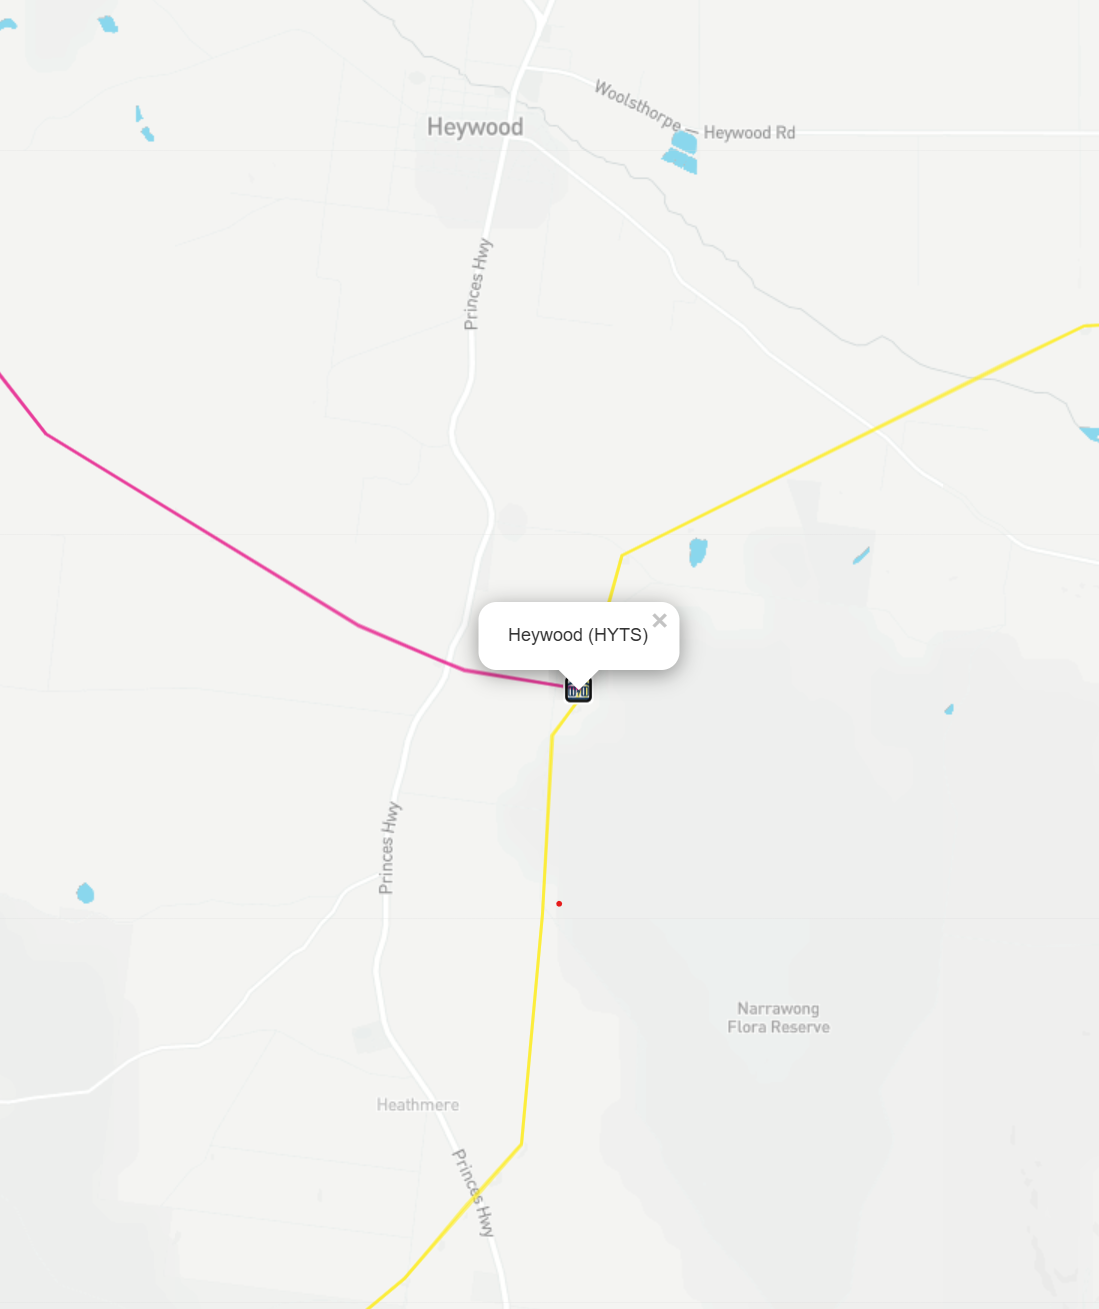
\includegraphics[width=0.7\textwidth]{\projectassetsdir/project-location.png} % Change example-image-a to the filename of your image
	\caption{Project location}
	\label{fig:project-location}
\end{figure}


	
	\chapter{Performance Standards}
	\section{[S5.2.5.1] Reactive Power Capability and Power Factor Requirements}
	\label{sec:s5251}
	\subsection{Automatic Access Standard}
	\begin{tcolorbox}[lightgreenbox]
		Integrated resource system's rated active power = 285 MW as measured at the Connection Point.

While operating at any level of active power output and at any voltage at the Connection Point within the limits of ±10\% of Normal Voltage, the integrated resource system is capable of supplying and absorbing at the Connection Point an amount of reactive power at least equal to the product of the rated active power of the integrated resource system and 0.395, as reflected in Figure 1.

\begin{figure}[H]
	\centering
	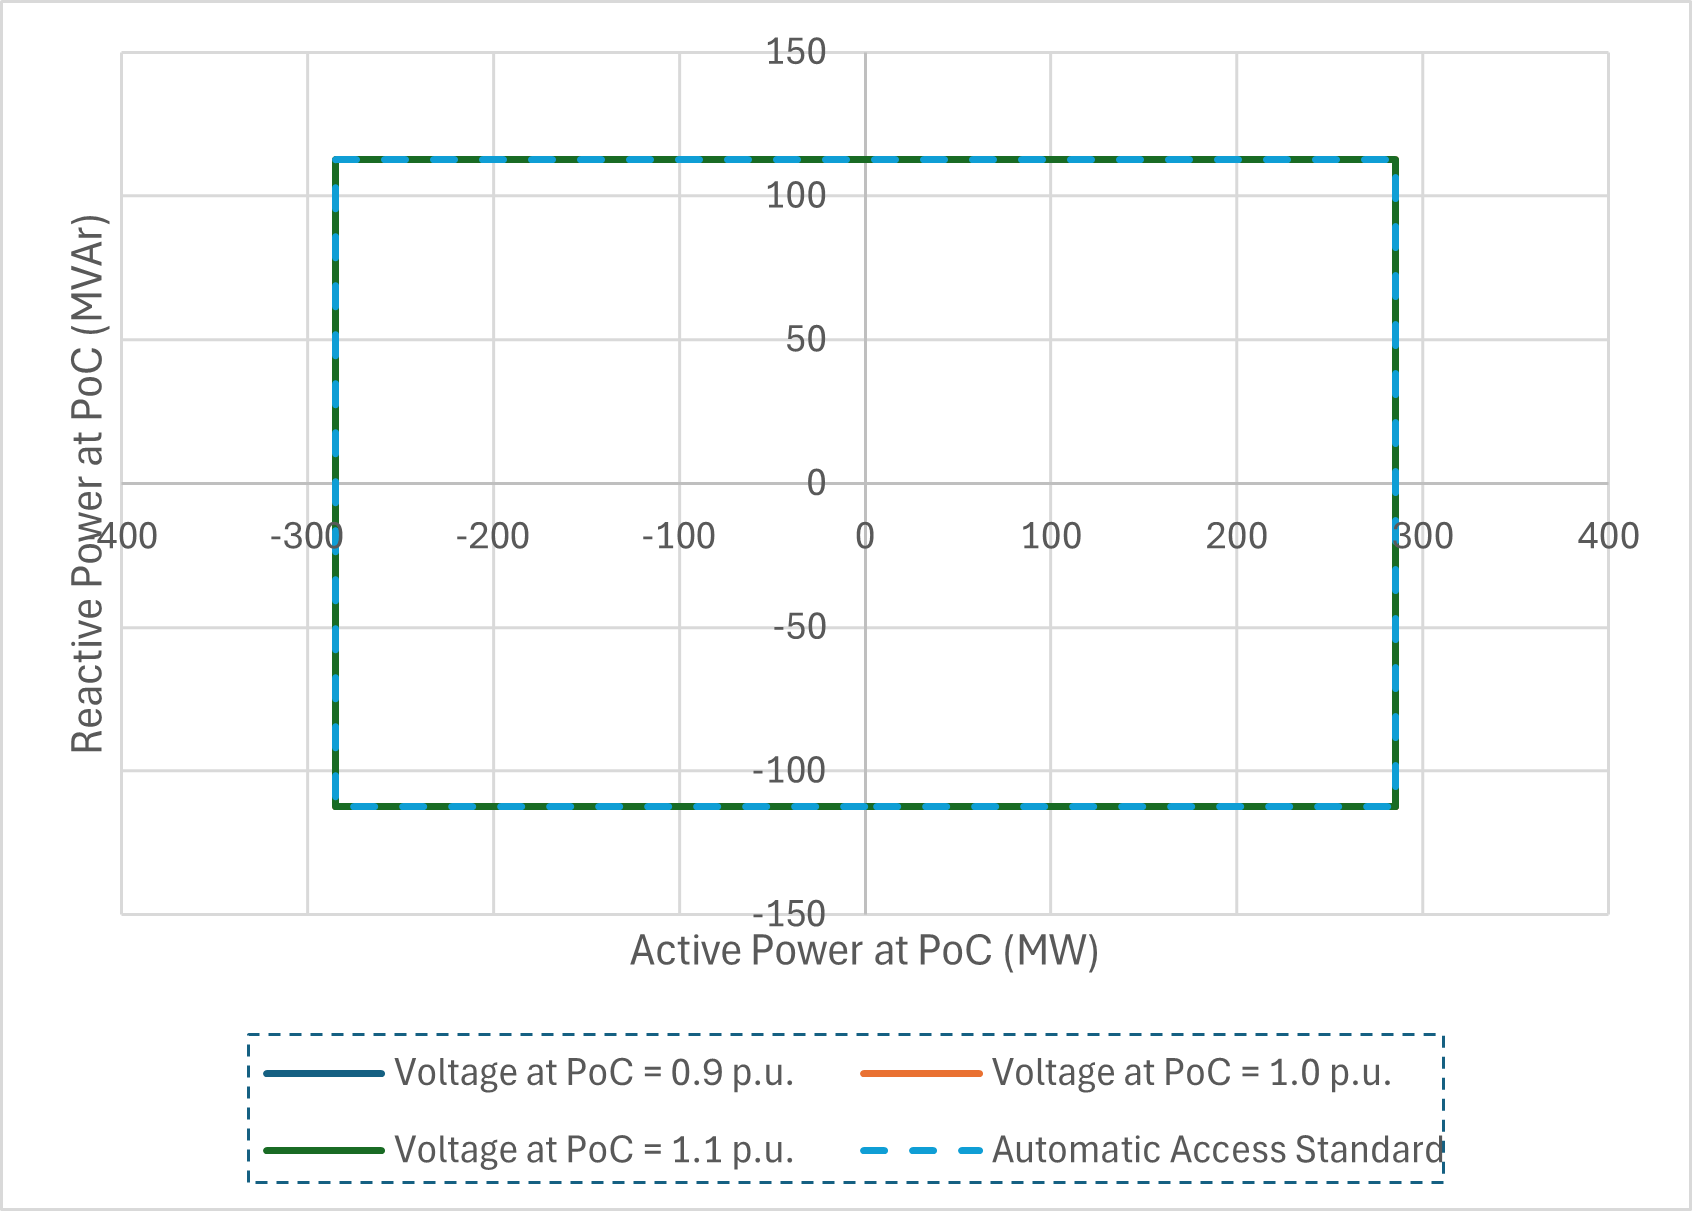
\includegraphics[width=0.8\textwidth]{\projectassetsdir/gps-clauses/s5251-curve.png}
\end{figure}
\textbf{Figure 1: Reactive power capability up to 50°C rating}

The integrated resource system, while not generating active power and not supplying or absorbing reactive power under an ancillary services agreement:
\begin{itemize}
	\item When the production units are connected and the ambient temperature is less than 50OC, follow the voltage regulation control requirement specified in the performance standard under clause S5.2.5.13 with a reactive power capability of ± 1.223 MVAr for each production unit; and
	\item When the production units are not connected, not supply at its Connection Point reactive power of more than 0 MVAr and not draw more electricity than XXXX kW of active power and XXXX kVAr of reactive power;
\end{itemize}

If the reactive power supplied or absorbed at the Connection Point falls outside the range that applies when the production units are not connected, the integrated resource system must, where required by the NSP in order to maintain satisfactory voltage levels at the Connection Point or to restore intra-regional or inter-regional power transfer capability, take action to ensure that the reactive power falls within that range within 30 min.

	\end{tcolorbox}
	\subsection{Assessment Methodology}
	Reactive capability studies have been performed on a full, detailed model of the plant (including 
	all cables, inverters and transformers), based on inverter reactive capability curves supplied by 
	the OEM. Powerfactory is capable of interpolating between these curves, allowing for accurate 
	reactive power output to be calculated based on the individual terminal voltages of each inverter\footnote{Note that Powerfactory is not capable of doing the same for active power, so invalid active power values are
		removed in post-processing.}.\\
	For each ambient temperature and connection point voltage to be studied, the appropriate capability curve for the inverter is applied and the connection point voltage is fixed to the target level. With the transformers permitted to tap, the case is first solved with all inverters exporting as much reactive power as possible without leaving their range of terminal voltages for which they are able to individually maintain Continuous Uninterrupted Operation (CUO). This study is repeated with all inverters importing as much reactive power as possible while maintaining CUO. Both processes are then repeated for all levels of inverter active power dispatch and a complete reactive capability curve is developed by recording the connection point active and reactive power outputs for all studies.\\
	To confirm CUO is maintained at a generating system level for s5.2.5.4, the same study is repeated, but prior to recording the results, the transformer On-Load Tap Changers (OLTCs) are then allowed to tap at most twice, and the connection point voltage is stepped to the extents of the CUO voltage band or ±10\%, 
	whichever is less onerous\footnote{Per AEMO recommended rule change.}. The results for these studies are recorded as alternative, more onerous ”CUO curves.”. A maximum of two taps was allowed for these tests as with a total time per tap of 10 seconds, the OLTC is actually capable of performing 6 taps in a given 60 second window. This ensures that the plant is able to "exit" the withstand regions seen in Figure \ref{fig:s5254-cuo-summary-pscad}, preventing tripping of the inverter and ensuring CUO is maintained. \\
	The remainder of the s5.2.5.1 clause consists of restrictions around the following:
	\begin{enumerate}[label=(\arabic*)]
		\item How much active and reactive power can be imported or exported by the generating system when the inverters are connected but not generating active power, which allows for the consideration of the inverters’ ability to provide reactive power when state of charge is maintained, but does not allow for the filters to be out of service as they are required to offset the harmonics produced by inverters. In the operations phase, this would be a time when the generator has bid out, is curtailed.
		
		\item When the inverters are disconnected, which allows for the disconnection of the harmonic filter and even the 33kV circuit breaker, as this would only occur if there was a significant problem with the control system or a planned maintenance outage of the whole generating system.
	\end{enumerate}
	\subsection{Results}
		The reactive capability curves for HEYWOODBESS at 35°C, 40°C and 50°C are shown in Figures \ref{fig:pq-curve-35degC}, \ref{fig:pq-curve-40degC} and \ref{fig:pq-curve-50degC}. Detailed results in .xslx format can be found in the Capability Curves folder.
	
	\begin{figure}[H]
		\centering
		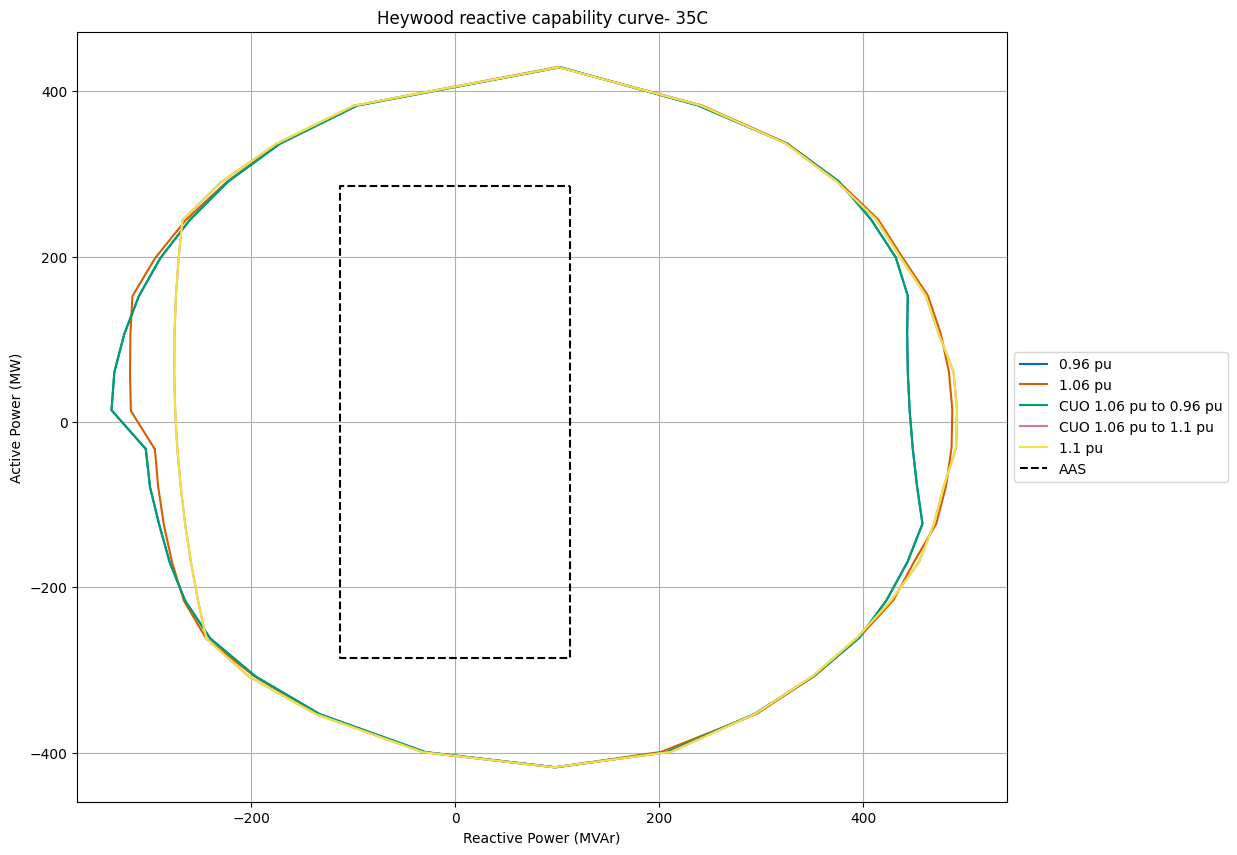
\includegraphics[width=0.8\textwidth]{\projectassetsdir/capability-curves/new_Heywood reactive capability curve- 35C.png}
		\caption{35°C Reactive capability curve for HEYWOODBESS}
		\label{fig:pq-curve-35degC}
	\end{figure}
	
	\begin{figure}[H]
		\centering
		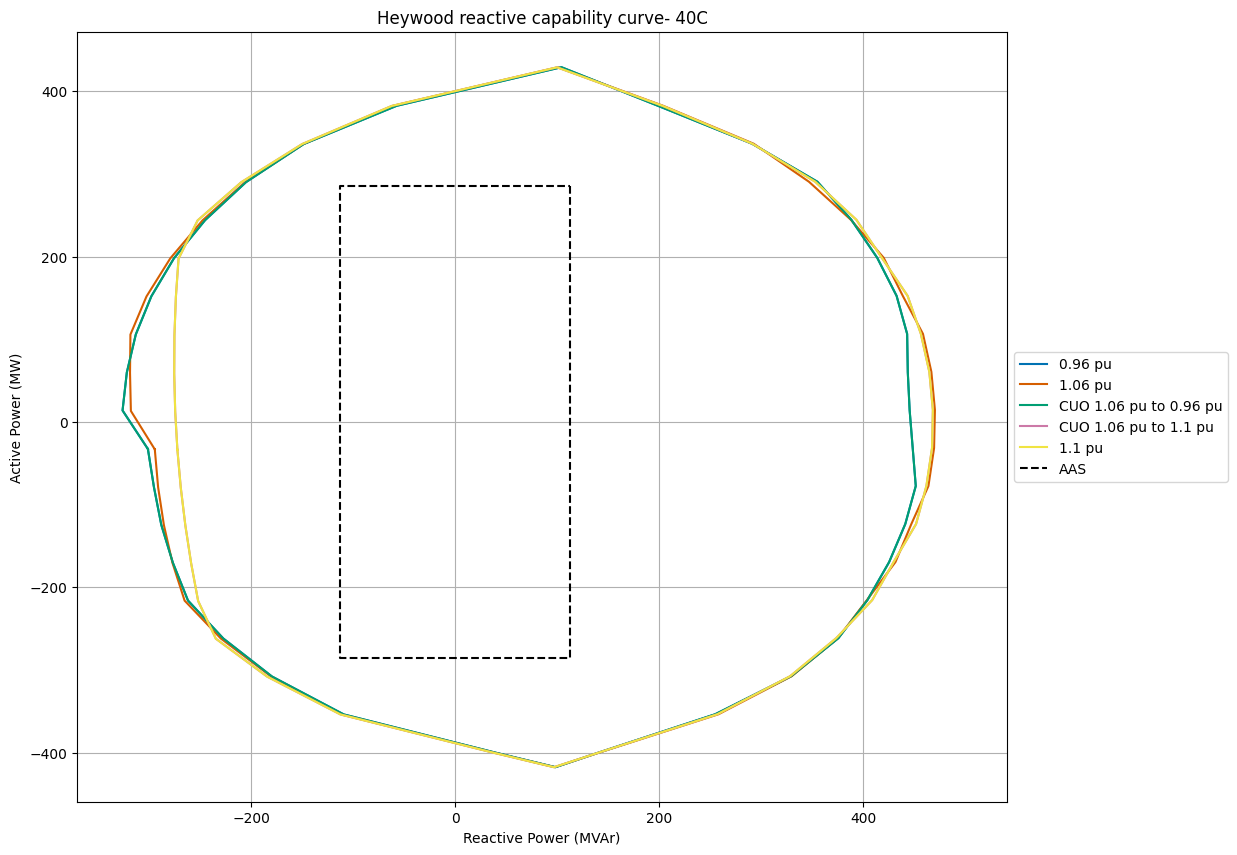
\includegraphics[width=0.8\textwidth]{\projectassetsdir/capability-curves/new_Heywood reactive capability curve- 40C.png}
		\caption{40°C Reactive capability curve for HEYWOODBESS}
		\label{fig:pq-curve-40degC}
	\end{figure}
	
	\begin{figure}[H]
		\centering
		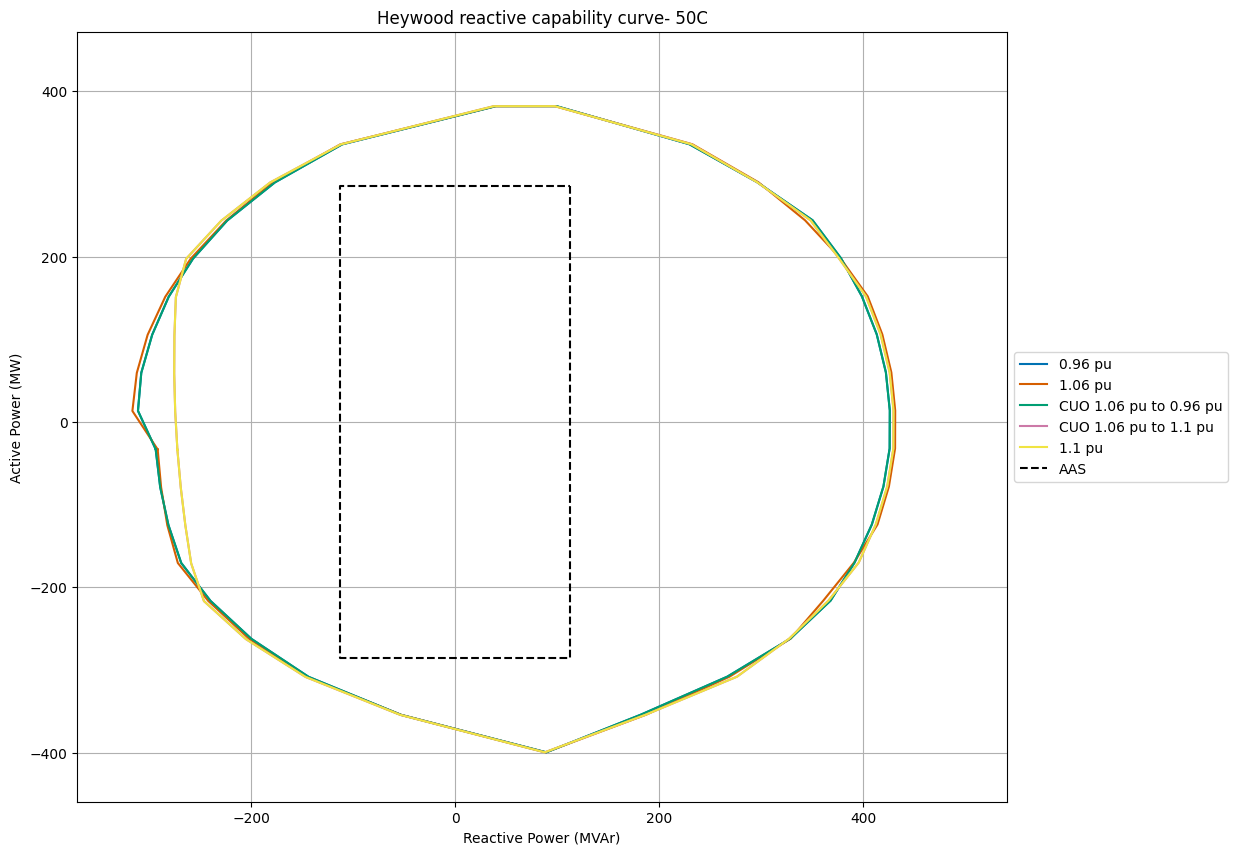
\includegraphics[width=0.8\textwidth]{\projectassetsdir/capability-curves/Heywood reactive capability curve- 50C.png}
		\caption{50°C Reactive capability curve for HEYWOODBESS}
		\label{fig:pq-curve-50degC}
	\end{figure}

	To assess compliance with the second part of this clause a study in PowerFactory was conducted to examine the power flow at the point of connection when auxiliary loads are connected, but the inverters and harmonic filters are disconnected. The results of this have been included in Table \ref{tab:5251-poc-flows} which demonstrate that Heywood BESS is compliant.
	
	\begin{table}[H]
		\centering
		\caption{Point of connection power flows}
		\label{tab:5251-poc-flows}
		\begin{tabular}{|l|c|c|c|c|}
			\hline
			\textbf{Status of Inverters} & \textbf{Status of Aux Loads}  & \textbf{Status of HFs} & \textbf{Power flow at the POC} \\
			\hline
			OFF & ON	& OFF & $P_{meas}$=1.5 MW, $Q_{meas}$=0 MVAr \\
			\hline
		\end{tabular}			
	\end{table}	
	
	
	\section{[S5.2.5.2] Quality of Electricity Generated and Balancing Load Current Voltage Fluctuations Harmonics and Voltage Notching}	
	\subsection{Automatic Access Standard}
	\begin{tcolorbox}[lightgreenbox]
		%\documentclass{article}
%\usepackage{graphicx}
%\begin{document}
	
	\begin{itemize}
		\item When generating and when not generating, the integrated resource system does not produce at the Connection Point:
		\begin{itemize}
			\item[(a)] Voltage fluctuations greater than the limits specified in Table 2.1 by the NSP under clause S5.1.5(a) of the NER, where flicker will be measured in accordance with AS/NZS 61000.3.7:2001:
		\end{itemize}
		
			\begin{center}
			\begin{tabular}{|c|c|}
				\hline
				\textbf{Pst} & \textbf{Plt} \\
				\hline
				0.35 & 0.25 \\
				\hline
			\end{tabular}
			\end{center}
		
		\begin{itemize}
			\item[(b)] Harmonic voltage distortion greater than the limits specified in Table 2.2 by the NSP under clause S5.1.6(a) of the NER and will be measured at the Connection Point in accordance with AS/NZS 61000.3.6:2001:
		\end{itemize}
		
			\begin{center}
			\begin{tabular}{|p{2cm}|p{2cm}|p{2cm}|p{2cm}|p{2cm}|p{2cm}|}
				\hline
				\textbf{Harmonic Order (h)} & \textbf{Harmonic Voltage Limits (\%)} & \textbf{Harmonic Order (h)} & \textbf{Harmonic Voltage Limits (\%)} & \textbf{Harmonic Order (h)} & \textbf{Harmonic Voltage Limits (\%)} \\
				\hline
				2 & 0.1 & 19 & 0.12 & 36 & 0.1 \\
				3 & 0.1 & 20 & 0.1 & 37 & 0.1 \\
				4 & 0.1 & 21 & 0.1 & 38 & 0.1 \\
				5 & 0.1 & 22 & 0.1 & 39 & 0.1 \\
				6 & 0.1 & 23 & 0.1 & 40 & 0.1 \\
				7 & 0.1 & 24 & 0.1 & 41 & 0.1 \\
				8 & 0.1 & 25 & 0.1 & 42 & 0.1 \\
				9 & 0.1 & 26 & 0.1 & 43 & 0.1 \\
				10 & 0.1 & 27 & 0.1 & 44 & 0.1 \\
				11 & 0.18 & 28 & 0.1 & 45 & 0.1 \\
				12 & 0.1 & 29 & 0.1 & 46 & 0.1 \\
				13 & 0.18 & 30 & 0.1 & 47 & 0.1 \\
				14 & 0.1 & 31 & 0.1 & 48 & 0.1 \\
				15 & 0.1 & 32 & 0.1 & 49 & 0.1 \\
				16 & 0.1 & 33 & 0.1 & 50 & 0.1 \\
				17 & 0.12 & 34 & 0.1 & THD & 0.23 \\
				18 & 0.1 & 35 & 0.1 & & \\
				\hline
			\end{tabular}
			\end{center}
		
		\begin{itemize}
			\item[(c)] Voltage unbalance greater than the limits specified in Table 2.3 by the NSP under clause S5.1.7(c) of the NER and will be measured in accordance with AS/NZS 61000.3.6:2001:
		\end{itemize}
		
			\begin{center}
			\begin{tabular}{|p{3cm}|p{2cm}|p{2cm}|p{2cm}|p{2cm}|}
				\hline
				\multirow{2}{*}{{\makecell{\textbf{Nominal Supply} \\ \textbf{Voltage (kV)}}}} & \multicolumn{4}{c|}{\textbf{Maximum Negative Sequence Voltage (\% of Nominal Voltage)}} \\ 
				\cline{2-5}
				& \textit{No contingency event} (30-min average) & \textit{Credible contingency event} (30-min average) & General (10-min average) & Once per hour (1-min average) \\ 
				\hline
				275 & 0.5 & 0.7 & 1.0 & 2.0 \\ 
				\hline
			\end{tabular}
			\end{center}
	\end{itemize}
	
%\end{document}

	\end{tcolorbox}
	\subsection{Assessment}
	The Harmonic Emissions Assessment and Filter Design is currently unavailable at the R0 stage.
	
	\section{[S5.2.5.3] Generating System Response to Frequency Disturbances}
	\subsection{Automatic Access Standard}
	\begin{tcolorbox}[lightgreenbox]
			Unless the rate of change of frequency is outside the range of ±4 Hz/s for more than 0.25 s, ±3 Hz/s for more than 1.00 s, the integrated resource system and each of its production units is capable of continuous uninterrupted operation for frequencies in the ranges indicated in Table 2.4:
	

	\begin{table}[H]
		\centering
		\begin{tabular}{|c|c|}
			\hline
			\textbf{Frequency Range (Hz)\textsuperscript{(1)}} & \textbf{Duration\textsuperscript{(1)}} \\ \hline
			47 to 48 & 2 min \\ \hline			
			48 to 49.5 & 10 min \\ \hline			
			49.5 to 50.5 & continuous \\ \hline
			50.5 to 52 & 10 min \\ \hline
		\end{tabular}
		\caption*{Table 2.4:  Frequency Limits for Continuous Uninterrupted Operation}
	\end{table}
	Notes:  
	
	\textsuperscript{(1)} Based on the frequency operating standard effective 1 January 2020.
	

	
	\end{tcolorbox}
	
	
	\subsection{Assessment Methodology}
	To assess this clause, a series of 'envelope' tests were performed, where the system frequency was initialised at 50Hz, then ramped to the furthest extent of the \ac{OFRT} or \ac{UFRT} ride-through bands, then gradually ramped down such that each band is sustained for the required duration. The results are then analysed to confirm that no generating units tripped during the study.

To implement these tests, $F_{\mathrm{grid}}$ is driven with a time-series signal $F_{\mathrm{grid}_{\mathrm{1}}}, F_{\mathrm{grid}_{\mathrm{2}}}, F_{\mathrm{grid}_{\mathrm{3}}}, \dots, F_{\mathrm{grid}_{\mathrm{n}}}$, as shown in Figure~\ref{fig:s5253-assessment-methodology}. The assessment is performed on an infinite grid.

\begin{figure}[H]
	\centering
	
	\newcommand{\bushere}[3]{% length, text above, text below}
	% Optional arguments do nto work in paths
	%
	% starting point; draw an edge and then two nodes
	% save the position
	coordinate(tmp)
	% go up and do an edge down
	++(0,#1) node[anchor=base, font=\footnotesize]{#2} edge[ultra thick] ++(0, {-2*#1})
	% edges do not move the current point, go down to position the node
	++(0,{-2*#1}) node[below]{#3}
	% go back to where we started
	(tmp)
	}
	
	\ctikzset{sources/fill=gray!20, resistors/fill=gray!20}
	\resizebox{0.7\linewidth}{!}{ % Set width to \linewidth
	\begin{tikzpicture}[semithick]% default line width
		% Buses and branches
		\draw (0,0)
		node[left, font=\footnotesize]{Generator} ++(1.5,0) \bushere{1.5}{Connection Point}{} coordinate(poc);
		\draw (poc) -- ++(1,0) node[vsourcesinshape, rotate=90]{} coordinate(vgrid) ++(0.5,0) node[right]{$V_{\text{grid}}$};
		\draw (poc) -- ++(-1,0) node[vsourcesinshape, rotate=90]{};
		% Fault
		\draw[blue, font=\footnotesize, <-] (vgrid) ++(0, -0.5) -- ++(0, -0.5) -- ++(0.5,0) node[right]{$F_{\mathrm{grid}_{\mathrm{1}}}, F_{\mathrm{grid}_{\mathrm{2}}}, F_{\mathrm{grid}_{\mathrm{3}}}, \dots, F_{\mathrm{grid}_{\mathrm{n}}}$};
		
	\end{tikzpicture}
	}	
	\caption{s5.2.5.3 assessment methodology}
	\label{fig:s5253-assessment-methodology}
\end{figure}
	
	All assessments for this clause have been performed in PSCAD.
	
	\subsection{Results}
	
	The under-frequency and over-frequency ride through performance of the generating system during the envelope tests (performed in PSCAD) relative to the agreed access standard is shown  in Figure \ref{fig:s5253-pscad-frt}. The project was able to remain connected and in continuous uninterrupted operation for the applied "envelope tests" to simulate the frequency withstand requirements of S5.2.5.3.  A summary of the envelope tests performed to produce this plot are shown in Table \ref{tab:s5253-test-suite}. The full results have been provided in Appendix \ref{Grid Frequency Disturbance Withstand Tests [S5.2.5.3]}. 
	
	\begin{figure}[H]
		\centering
		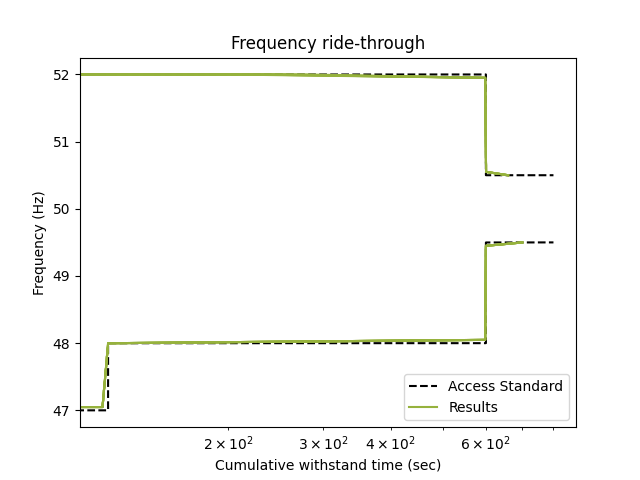
\includegraphics[width=0.7\textwidth]{\analysisdir/pscad/s5253_ride_through_results.png}
		\caption{Frequency ride-through performance}
		\label{fig:s5253-pscad-frt}
	\end{figure}

	
	\begin{table}[H]
		\centering
		\caption{s5.2.5.3 frequency ride-through test suite}
		\label{tab:s5253-test-suite}
		\autoscaledtable{H}{\projectassetsdir/test-suite-tables/CSR/5253-test-table.csv}
	\end{table}
	
	\section{[S5.2.5.4] Generating System Response to Voltage Disturbances}
	\subsection{Automatic Access Standard}
	\begin{tcolorbox}[lightgreenbox]
		The integrated resource system and each of its production units is capable of continuous uninterrupted operation where a power system disturbance causes the voltage at the Connection Point to vary within the ranges indicated in Table 2.5:

\begin{table}[H]
	\centering
	\resizebox{0.6\textwidth}{!}{%
		\begin{tabular}{|c|c|}
			\hline
			\textbf{Voltage Range (\% of Normal Voltage)} & \textbf{Duration} \\ \hline
			
			>130\% & 0.02 s\textsuperscript{(1)} \\ \hline
			125\% to 130\% & 0.2 s\textsuperscript{(1)} \\ \hline
			120\% to 125\% & 2 s\textsuperscript{(1)} \\ \hline
			115\% to 120\% & 20 s\textsuperscript{(1)} \\ \hline
			110\% to 115\% & 20 mins\textsuperscript{(1)} \\ \hline
			90\% to 110\% & continuous \\ \hline
			80\% to 90\% & 10 s\textsuperscript{(2)} \\ \hline
			70\% to 80\% & 2 s\textsuperscript{(2)} \\ \hline			
		\end{tabular}
	}
	\caption*{Table 2.5: Voltage Limits for Continuous Uninterrupted Operation}
\end{table}
Notes:

\textsuperscript{(1)} After the Connection Point voltage first varied above 110\% of Normal Voltage before returning to between 90\% and 110\% of Normal Voltage.

\textsuperscript{(2)} After the Connection Point voltage first varied below 90\% of Normal Voltage before returning to between 90\% and 110\% of Normal Voltage.

	\end{tcolorbox}
	
	\subsection{Assessment Methodology}
	\label{s5254-method}
	S5.2.5.4 tests assess the ability of the generator to ride-through and maintain \ac{CUO} to a changing Connection Point voltage.

Three types of studies are run:

\begin{enumerate}
	\item "Envelope" tests, where the Connection Point voltage is initialised to a normal value, then stepped up to the furthest extent of the \ac{UVRT} or \ac{OVRT} ride-through bands, then gradually stepped down such that each band is sustained for the required duration. 
	\item "Withstand" tests, where the Connection Point voltage is initialised to a normal value, then stepped to the furthest extent of one of the ride-through bands and held for the required withstand time.
	\item \ac{CUO} studies, where the Connection Point voltage is initialised to a normal value, then stepped to 0.9pu (or 0.1pu lower than the initial voltage, whichever is higher) or to 1.1pu (or 0.1pu higher than the initial voltage, whichever is lower). These studies test the ability of the generator to maintain $P_{\mathrm{POC}_{\mathrm{pre-fault}}}$ and $Q_{\mathrm{POC}_{\mathrm{pre-fault}}}$ after the disturbance.
\end{enumerate}

To perform these tests, $V_{\mathrm{grid}_{\mathrm{1}}}$ is selected to correspond to the required $V_{\mathrm{POC}_{\mathrm{1}}}$, as these studies are performed on an infinite grid. Subsequent $V_{\mathrm{grid}}$ values $V_{\mathrm{grid}_{\mathrm{2}}}, V_{\mathrm{grid}_{\mathrm{3}}}, \dots, V_{\mathrm{grid}_{\mathrm{n}}}$ can then be chosen to match the desired $V_{\mathrm{POC}}$ values $V_{\mathrm{POC}_{\mathrm{2}}}, V_{\mathrm{POC}_{\mathrm{3}}}, \dots, V_{\mathrm{POC}_{\mathrm{n}}}$ values for the test, as shown in Figure~\ref{fig:s5254-assessment-methodology}.

\begin{figure}[H]
	\centering
	\newcommand{\bushere}[3]{% length, text above, text below}
% Optional arguments do nto work in paths
%
% starting point; draw an edge and then two nodes
% save the position
coordinate(tmp)
% go up and do an edge down
++(0,#1) node[anchor=base, font=\footnotesize]{#2} edge[ultra thick] ++(0, {-2*#1})
% edges do not move the current point, go down to position the node
++(0,{-2*#1}) node[below]{#3}
% go back to where we started
(tmp)
}

\ctikzset{sources/fill=gray!20, resistors/fill=gray!20}
\resizebox{0.5\linewidth}{!}{ % Set width to \linewidth
	\begin{tikzpicture}[semithick]% default line width
		% Buses and branches
		\draw (0,0)
		node[left, font=\footnotesize]{Generator} ++(1.5,0) \bushere{1.5}{Connection Point}{} coordinate(poc);
		% One load (start from the coord load, go up)
		\ctikzset{bipoles/border margin=0.5}% See manual section 3.1.2
		\draw (poc) -- ++(1,0) node[vsourcesinshape, rotate=90]{} coordinate(vgrid) ++(0.5,0) node[right]{$V_{\text{grid}}$};
		\draw (poc) -- ++(-1,0) node[vsourcesinshape, rotate=90]{};
		% Fault
		\draw[blue, font=\footnotesize, <-] (vgrid) ++(0, -0.5) -- ++(0, -0.5) -- ++(0.5,0) node[right]{$V_{\mathrm{grid}_{\mathrm{1}}}, V_{\mathrm{grid}_{\mathrm{2}}}, V_{\mathrm{grid}_{\mathrm{3}}}, \dots, V_{\mathrm{grid}_{\mathrm{n}}}$};
		
	\end{tikzpicture}
}






	\caption{Grid voltage disturbance methodology}
	\label{fig:s5254-assessment-methodology}
\end{figure}
	
	All assessments for this clause have been performed in PSCAD.
	
	\subsection{Results}
	The under-voltage and over-voltage ride through performance of the generating system during the envelope tests relative to the agreed access standard is shown in Figure \ref{fig:s5254_ride_through_results}. This plot illustrates the connection point voltage for all envelope tests over simulation time. Please refer to results of the envelope tests in Appendix \ref{tab:s5254-envelope-and-withstand-test-suite}, which demonstrate that the solar farm was able to remain connected for at least the duration required by the access standard through simulation \footnote{Please note that for the first HVRT step down to 1.3pu the reason the trace is seen to be thicker for this segment is because several envelope test results have been overlayed, which have small variations in point of connection voltage}.

	
	\begin{figure}[H]
		\centering
		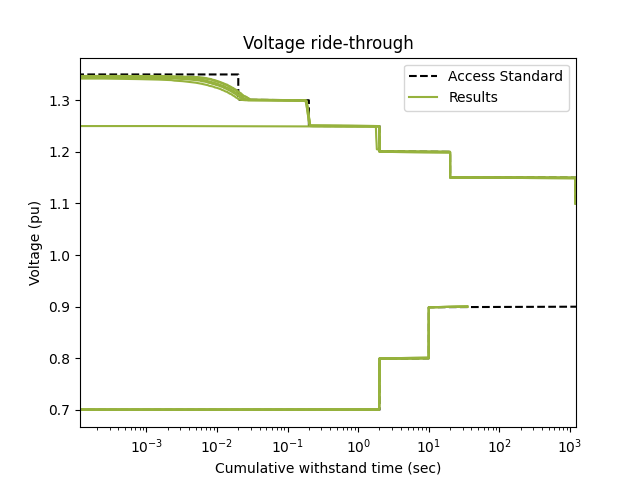
\includegraphics[width=0.7\textwidth]{\analysisdir/pscad/s5254_ride_through_results.png}
		\caption{Over-voltage ride-through performance}
		\label{fig:s5254_ride_through_results}
	\end{figure}
	

	{
		\fontsize{7}{9}\selectfont
		\autoscaledlongtable
		{s5.2.5.4 envelope withstand test suite}
		{tab:s5254-envelope-and-withstand-test-suite}
		{\projectassetsdir/test-suite-tables/CSR/5254-Withstand-test-table.csv}
	}
	
	The ability of the generating system and the individual generating units to maintain \ac{CUO} can be confirmed through the combination of the following: reactive capability studies (presented in \ref{sec:s5251}) and the chart in Figure \ref{fig:s5254-cuo-summary-pscad}, which shows that the inverter terminal voltages settle within the continuous operating limits prior to any protection timers operating for all \ac{CUO} test cases in Table \ref{tab:s5254-cuo-test-suite}. All test cases have been overlayed on the plot to demonstrate that all inverters settle to within their continuous operating voltage limits for all \ac{CUO} tests.

	\begin{figure}[H]
		\centering
		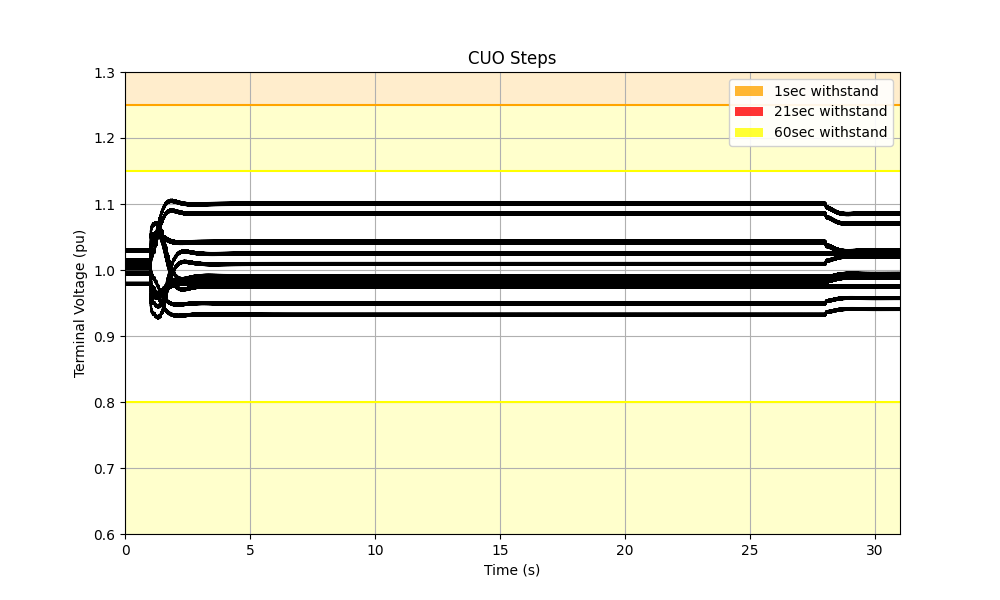
\includegraphics[width=0.9\textwidth]{\analysisdir/pscad/cuo_summary.png}
		\caption{Inverter CUO performance summary plot (PSCAD)}
		\label{fig:s5254-cuo-summary-pscad}
	\end{figure}
	


	Please refer to Appendix \ref{Continuous Uninterrupted Operation [S5.2.5.4]} which includes the results for each test.
	{
		\fontsize{7}{9}\selectfont
		\autoscaledlongtable
		{s5.2.5.4 CUO test suite (PSCAD)}
		{tab:s5254-cuo-test-suite}
		{\projectassetsdir/test-suite-tables/CSR/5254-CUO-test-table.csv}
	}

	\section{[S5.2.5.5] Generating System Response to Disturbances Following Contingency Events}
	\subsection{Negotiated Access Standard}
	\begin{tcolorbox}[lightgreenbox]
		For the purposes of this performance standard, a \textbf{fault} includes a fault of the relevant type having a metallic conducting path. 
Fault clearance times for relevant equipment are specified in Table 2.6:

	\begin{table}[H]
	\centering
	\begin{tabular}{|c|p{8cm}|}
		\hline
		\textbf{System} & \textbf Transmission system fault clearance time \\ \hline
		Primary protection system & 100 ms \\ \hline
		Breaker fail protection system & 250 ms \\ \hline
		Automatic reclose equipment & 
		Three-phase auto-reclose with 3-second deadtime and 1 shot \\ \hline
	\end{tabular}
	\caption*{Table 2.6: Protection clearance times in transmission and distribution system}
	\end{table}

\textbf{Single disturbance (reflects clause S5.2.5.5(c) of the NER):}  
Provided that the event is not one that would disconnect the integrated resource system from the power system by removing network elements from service, the integrated resource system and each of its production units will remain in continuous uninterrupted operation for any disturbance caused by:
\begin{enumerate}
	\item A credible contingency event;
	\item A three-phase fault in a transmission system cleared by all relevant primary protection systems;
	\item A two-phase-to-ground, phase-to-phase or phase-to-ground fault in the transmission system cleared in:
	\begin{enumerate}
		\item the longest time expected to be taken for a relevant breaker fail protection system to clear the fault or
		\item if a breaker fail protection system is not installed, the greater of the time specified in Table 2.7;
	\end{enumerate}
\end{enumerate}
		
		\begin{table}[H]
		\centering
		\begin{tabular}{|c|p{8cm}|}
			\hline
			\textbf{Nominal voltage at fault location (kV)} & \textbf{Time (ms)} \\ \hline
			>400 kV & 175 ms \\ \hline
			>250 kV and <400 kV & 250 ms \\ \hline
			>100 kV and <250 kV & 430 ms \\ \hline
			<100 kV & 430 ms \\ \hline
		\end{tabular}
		\caption*{Table 2.7: Fault Clearance Times}
		\end{table}

		and the longest time expected to be taken for all relevant primary protection systems to clear the fault.
\begin{enumerate}
	\setcounter{enumi}{3}
	\item A three-phase, two-phase-to-ground, phase-to-phase or phase-to-ground fault in a distribution network cleared in:
	\begin{enumerate}[label=\roman*]
		\item the longest time expected to be taken for a relevant breaker fail protection system to clear the fault; or
		\item if a breaker fail protection system is not installed, the greater of 430 ms and the longest time expected to be taken for all relevant primary protection systems to clear the fault.
	\end{enumerate}
\end{enumerate}

\textbf{Multiple disturbances (reflects clause S5.2.5.5(d), (s), and (t) of the NER):}  
When assessing multiple disturbances, a fault that is re-established following operation of automatic reclose equipment is counted as a separate disturbance.  
The integrated resource system and each of its production units will remain in continuous uninterrupted operation for a series of up to 15 disturbances within any 5-min period caused by any combination of the events described above where:
\begin{enumerate}
	\item Up to 6 disturbances cause the Connection Point voltage to drop below 50\% of Normal Voltage; 
	\item In parts of the network where three-phase automatic reclosure is permitted, up to two disturbances are three-phase faults, and otherwise up to one three-phase fault where the Connection Point voltage drops below 50\% of Normal Voltage; 
	\item Up to one disturbance is cleared by a breaker fail protection system or similar backup protection system; 
	\item Up to one disturbance causes the Connection Point voltage to vary within the ranges under clause S5.2.5.4(a)(7) and (8) of the NER; 
	\item The minimum clearance from the end of one disturbance and commencement of the next disturbance may be zero milliseconds; and 
	\item All remaining disturbances are caused by faults other than three-phase faults, provided that none of the events would result in:
	\item The islanding of the integrated resource system or cause a material reduction in power transfer capability by removing network elements from service; 
	\item The cumulative time that the Connection Point voltage is lower than 90\% of Normal Voltage exceeding 1,800 milliseconds within any 5-min period; or 
	\item Within any 5-min period, the time integral of the difference between 90\% of Normal Voltage and the Connection Point voltage when the Connection Point voltage is lower than 90\% of Normal Voltage exceeding 1 pu second.
The integrated resource system will not, as a consequence of its connection, cause other generating plant or loads to trip as a result of an event, when they would otherwise not have tripped for the same event.
\end{enumerate}

\textbf{For asynchronous integrated resource systems (reflects clause S5.2.5.5(f)-(i) and (u) of the NER):}  
Subject to any changed power system conditions or energy source availability beyond the Integrated Resource Provider's reasonable control, the integrated resource system, including all operating asynchronous production units (in the absence of a disturbance), in respect of fault types described in clause S5.2.5.5(c)(2) to (4) of the NER, will supply to, or absorb from, the network:

\begin{enumerate}
	\item During the disturbance and maintained until the Connection Point voltage recovers to between 90\% and 110\% of Normal Voltage, to assist the maintenance of power system voltages during the fault:
	\begin{enumerate}
		\item Capacitive reactive current in addition to its pre-disturbance level of at least 2.94\% of the maximum continuous current for each 1\% reduction of the Connection Point voltage below the range of  85\% to 90\% of Normal Voltage up to the maximum continuous current; 
		\item Inductive reactive current in addition to its pre-disturbance level of at least 3.1\% of its maximum continuous current for each 1\% increase of the Connection Point voltage above the range of 110\% to 115\% of Normal Voltage up to its maximum continuous current to maintain its rated apparent power; and

		\item the reactive current response will have a rise time of no greater than 40 ms and a settling time of no greater than 133 ms and will be adequately damped; and
		\item the reactive current contribution is calculated using sequence components
	\end{enumerate}
	\item from 230 ms after clearance of the fault, active power of at least 95\% of the level existing just prior to the fault. 
\end{enumerate}

	\end{tcolorbox}
	\subsection{Assessment Methodology}
	Assessment of s5.2.5.5 is performed in by applying a variety of different types of faults with different impedances to observe the generating system response and measure characteristics such as settling times and $i_{\text{q}}$ injection performance. 

In PSCAD and PSSE SMIB studies, faults are applied to the connection point (as shown in Figure~\ref{fig:s5255-fault-application-methodology-diagram}) with characteristics that are representative of how real world faults would appear from the generating system's connection point, while in PSSE wide area studies, faults with credible characteristics are applied to the real network assets.

\begin{figure}[H]
	\centering
	\newcommand{\bushere}[3]{% length, text above, text below}
% Optional arguments do nto work in paths
%
% starting point; draw an edge and then two nodes
% save the position
coordinate(tmp)
% go up and do an edge down
++(0,#1) node[anchor=base, font=\footnotesize]{#2} edge[ultra thick] ++(0, {-2*#1})
% edges do not move the current point, go down to position the node
++(0,{-2*#1}) node[below]{#3}
% go back to where we started
(tmp)
}

\ctikzset{sources/fill=gray!20, resistors/fill=gray!20}
\resizebox{0.65\linewidth}{!}{ % Set width to \linewidth
	\begin{tikzpicture}[semithick]% default line width
		% Buses and branches
		\draw (0,0)
		node[left, font=\footnotesize]{Generator} ++(1.5,0) \bushere{1.5}{Connection Point}{} coordinate(poc);
		\draw (poc)
		-- ++ (1,0) to[generic, l={$Z_{\text{grid}}$}, resistors/width=2] ++ (4,0)
		-- ++ (1,0)
		\bushere{1.5}{Infinite Bus}{} coordinate(infinite bus);
		% One load (start from the coord load, go up)
		\ctikzset{bipoles/border margin=0.5}% See manual section 3.1.2
		\draw (infinite bus) -- ++(1,0) node[vsourcesinshape, rotate=90]{} ++(0.5,0) node[right]{$V_{\text{grid}}$};
		\draw (poc) -- ++(-1,0) node[vsourcesinshape, rotate=90]{};
		% Fault
		\draw[red, font=\footnotesize] (poc) ++(0, -0.7) -- ++(0.7,0) -- ++(0,-1) node[ground]{} ++(0.6,0.2) node[]{$Z_{\text{fault}}$};
		
	\end{tikzpicture}
}






	\caption{SMIB fault application methodology}
	\label{fig:s5255-fault-application-methodology-diagram}
\end{figure}

In addition to faults, \ac{TOV} scenarios are studied in PSCAD SMIB by tapping a dummy transformer connected between the point of connection and the grid impedance in order to push the voltage at the point of connection up to a specific value. This allows finer control of the disturbance seen at the point of connection, as the voltage drop across the grid impedance doesn't need to be considered.

In order to assess the impact of the project on the South Australian electrical network, four wide area cases were prepared based on recommendations provided by ElectraNet. Descriptions of the four cases are available in Section \ref{sec:s52512} [S5.2.5.12] Impact on Network Capability. 

%For each case, the interconnector flows are characterised by the below.
%
%\begin{enumerate}
%	\item SA light load - Interconnectors exporting 850 MW. Barker Inlet and Snapper Point in service.
%	\item SA light-medium load - Interconnectors exporting 850 MW. Barker Inlet, Snapper Point, and QPS 5 in service.
%	\item SA medium-high load - Interconnectors importing 750 MW. Barker Inlet, Snapper Point, Pelican unit \#1, and QPS 5 in service.
%	\item SA high load - Interconnectors importing 1,300 MW. Barker Inlet, Snapper Point, Pelican units \#1 and \#2, and QPS 5 in service.
%\end{enumerate}
%
%The interconnectors and corresponding limits applicable to this project have been prepared below.
%
%\begin{table}[H]
%	\centering
%	\begin{tabular}{|c|c|c|}
%		\hline
%		Interconnector & Flow direction & Nominal Capacity (MW) \\ \hline
%		Heywood (VIC-SA) & Towards VIC & 550 \\ \hline
%		Heywood (VIC-SA) & Towards SA & 600 \\ \hline
%		PEC (SA-VIC-NSW) & Towards NSW & 800 \\ \hline
%		PEC (SA-VIC-NSW) & Towards SA & 800 \\ \hline
%		Murraylink (VIC-SA) & Towards Vic & 200 \\ \hline
%		Murraylink (VIC-SA) & Towards SA & 220 \\ \hline
%	\end{tabular}
%	\caption{Interconnector flows applicable to this project}
%	\label{tab:case-interconnector-flow}
%\end{table}
%The list of faults evaluated in WAN studies was limited to those studied as part of R0 - as directed by ElectraNet.
%
%Faults were carried out using AEMO's OPDMS snapshots, which incorporated nearby generation and the generator SMIB model, and evaluated performance of the generator for disturbances on the wide area network. A variety of faults were tested, including:
%
%\begin{itemize}
%	\item Three-phase-to-ground faults with circuit breaker failure clearance times
%	\item Two-phase-to-ground faults
%\end{itemize}

	
	All SMIB assessments for this clause have been performed in PSCAD and all wide-area contingency assessments have been performed in PSS/E.
	
	\subsection{Results}
	
	
	\subsubsection{SMIB studies}
	The list of faults performed in SMIB studies has been provided in Tables \ref{tab:s5255-smib-bal-fault-test-suite-pscad} and \ref{tab:s5255-smib-unbal-fault-test-suite-pscad}.

	
	Figure \ref{fig:5255-pscad-pos-diqdv-poc} shows the amount of positive and negative sequence $i_{\text{q}}$ injection at the inverter terminals to the change in connection point voltage across all faults studied. It can be read as follows:
	
	\begin{itemize}
		\item Grey circles indicate that the generating system is supplying more than the \textit{maximum continuous current} of the generating system\footnote{The current associated with maximum active power and maximum reactive power while at 1.0pu voltage.}, which automatically fulfills the GPS requirement for reactive current injection, regardless of the additional $i_{\text{q}}$ injected.
		\item Red markers indicate the amount of additional $i_{\text{q}}$ injected for a particular fault. For compliance, the marker should be above the access standard characteristic (for faults) or below the characteristic (for \ac{TOV} tests).
	\end{itemize}
	
	We note that for all tests studied, the generating system was capable of providing sufficient positive sequence reactive current.
	\begin{figure}[H]
		\centering
		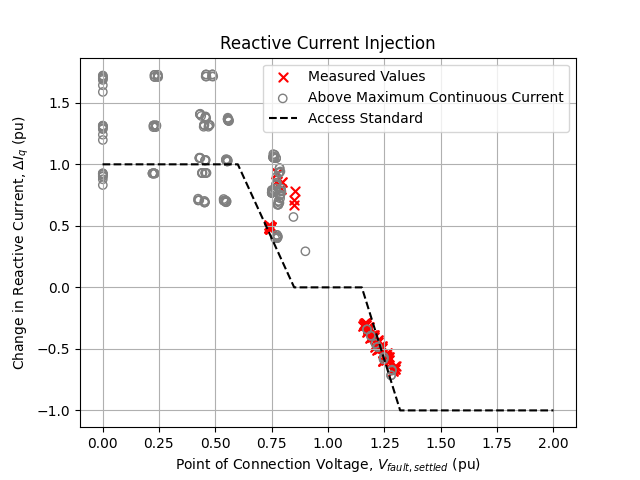
\includegraphics[width=0.8\textwidth]{\analysisdir/pscad/diqdv_characteristic.png}
		\caption{POC Positive Sequence Reactive Current Injection Performance}
		\label{fig:5255-pscad-pos-diqdv-poc}
	\end{figure}
	

	
	The full list of balanced faults, unbalanced faults, and TOV tests assessed can be found in Tables \ref{tab:s5255-smib-bal-fault-test-suite-pscad}, \ref{tab:s5255-smib-unbal-fault-test-suite-pscad}, and \ref{tab:s5255-smib-tov-test-suite-pscad} respectively.
	
	
	{
		\fontsize{6.5}{9}\selectfont
		\autoscaledlongtable
		{s5.2.5.5 balanced fault test suite (PSCAD)}
		{tab:s5255-smib-bal-fault-test-suite-pscad}
		{\projectassetsdir/test-suite-tables/CSR/5255-balFaults-test-table.csv}
	}
	
	{
		\fontsize{6.5}{9}\selectfont
		\autoscaledlongtable
		{s5.2.5.5 unbalanced fault test suite (PSCAD)}
		{tab:s5255-smib-unbal-fault-test-suite-pscad}
		{\projectassetsdir/test-suite-tables/CSR/5255-UnbalFaults-test-table.csv}
	}

	{
		\fontsize{7}{9}\selectfont
		\autoscaledlongtable
		{s5.2.5.5 TOV test suite (PSCAD)}
		{tab:s5255-smib-tov-test-suite-pscad}
		{\projectassetsdir/test-suite-tables/CSR/5255-TOV-test-table.csv}
	}

	The corresponding $i_{\text{q}}$ rise time, settle time and active power recovery times have been prepared below. Analysis was undertaken across all balanced and unbalanced faults in order to determine the positive and negative sequence current rise and settle times, in addition to the generating systems active power recovery time. Please refer to Table \ref{tab:s5255-smib-fault-test-suite-analysis-pscad}. 
	
	All faults were found to be compliant with the requirement for a 40ms $i_{\text{q}}$ rise time. For faults entering FRT, 15 faults have a settling time greater than 70ms, and 198 faults are slightly over 70ms, with the maximum settling time being 132ms.
	
	For a select number of temporary over-voltage and balanced/unbalanced faults, the reactive current settle time was found to exceed 70ms. By examining the reactive current waveform for these tests we see that there is a spike in reactive current approximately 80ms into the disturbance. The calculation for reactive current settle time is sensitive to this behaviour and as a consequence we arrive at a value larger than 70ms. This behaviour has been queried with SMA to which SMA has confirmed that this phenomenon is known and unavoidable. The spike introduced shortly after application of the disturbance is due to the Phase-Locked Loop (PLL) responding to changes in the network voltage phase angle. While PLLs can be tuned, it is SMAs advice that regardless of the parameters selected for the PLL mechanism, signal filtering will always be required and therefore some time delays in obtaining the phase angle of the network during fast transients will always be present. Please refer to SMAs technical memo on this subject \cite{sma-iq-settle}. This phenomenon will be discussed further with ElectraNet to understand whether it requires an amendment the exiting GPS or whether it is understood to be a modelling artifact. 
	
	

	{
		\fontsize{6.5}{7}\selectfont
		\autoscaledlongtable
		{s5.2.5.5 Fault test suite analysis (PSCAD)}
		{tab:s5255-smib-fault-test-suite-analysis-pscad}
		{\analysisdir/pscad/S5255 POC Faults Rise Settle Recovery Analysis/s5255_rise_settle_recovery_times.csv}
	}

	

	
	\subsubsection{Multiple fault disturbances}
	Compliance to the MFRT requirements of this clause have been demonstrated in PSCAD SMIB. The test suite defined in Section 3.2.6 of the PSCAD Dynamic Model Acceptance Test Guideline (DMAT) \cite{dmat-guideline} was performed and supporting results have been provided with the pscad dmat report \cite{pscad-mfrt-dmat}. All tests demonstrate that HEYWOOD BESS was capable of riding through all applied successive faults. Additionally, please refer to the provided letter of NER compliance \cite{ner-compliance} provided by SMA which confirms the ride through capability of the inverters for successive faults.
	
	
	
	\subsubsection{WAN studies}
	\label{subsubsec:WAN-results}
	%	Generators in the vicinity of Goorambat East Solar Farm were solved in accordance with their reactive power control mode. This ensures that the recorded network voltages are more in line with what would be expected in reality at steady state. These control modes and corresponding setpoints have been provided in the table below.
%	
%	\begin{table}[H]
%		\centering
%		\caption{Nearby large scale generator reactive power control modes and setpoints.}
%		\label{tab:control-modes}
%		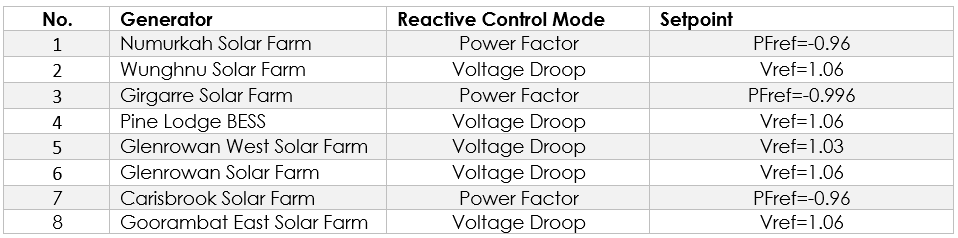
\includegraphics[width=0.8\textwidth]{report-assets/case information/generator_control_modes.png}
%	\end{table}
	%\newpage
	The list of faults evaluated in WAN studies was limited to those studied as part of R0 - as directed by ElectraNet. The 3phg faults,2phg faults with circuit breaker failure (CBF) timings (as per NER Table S5.1a.2), and 1phg faults with auto-reclose to nearby fault contingencies considered for the wide area network assessment are summarised in the table below. \ref{tab:wide-area-contingencies}. Please note that for contingencies 37–43, which are trip tests, faults are applied to trip transformers or generators in order to assess their impact on the system.

	
	{
		\fontsize{7}{9}\selectfont
		\autoscaledlongtable
		{Wide area studies test suite (PSSE) - Line Contingencies}
		{tab:wide-area-contingencies}
		{\projectassetsdir/test-suite-tables/General-Contingencies-test-table.csv}
	}
	
	The trip contingencies are summarised in Tables \ref{tab:Other-Contingencies}.
	{
		\fontsize{7}{9}\selectfont
		\autoscaledlongtable
		{Wide area studies test suite (PSSE) - Other Contingencies}
		{tab:Other-Contingencies}
		{\projectassetsdir/test-suite-tables/Other-Contigencies.csv}
	}

	
	As these faults were tested on the wide area network, they were generally less severe than the most severe faults tested in the SMIB environment, which left no retained voltage at the point of connection. These faults have been analysed to determine the stability of the model, and the network, including the ability to recover to a stable operating point following the contingency.
	
	
	
	The integrated resource system performed well in all disturbances tested, with the network voltage control not being negatively impacted by the presence of Heywood BESS. The results for each case have been prepared in Appendices \ref{WAN Case 1 - Wide Area Network Contingency Results [S5.2.5.5]} through \ref{WAN Case 4 - Wide Area Network Contingency Results [S5.2.5.5]}.
	
	
	\section{[S5.2.5.6] Quality of Electricity Generated and Continuous Uninterrupted Operation}
	\subsection{Negotiated Access Standard}
	\begin{tcolorbox}[lightgreenbox]
		The integrated resource system and each of its operating production units and reactive plant, will not disconnect from the power system for voltage fluctuation, harmonic voltage distortion and voltage unbalance at the Connection Point within the levels specified:
\begin{enumerate}
	\item For voltage fluctuations at the Connection Point, in the "compatibility levels" set out in Table 1 of AS/NZS 61000.3.7:2001.
	\item For harmonic voltage distortion at the Connection Point, in the "compatibility levels" defined in Table 1 of AS/NZS 61000.3.6:2001.
	\item For a negative sequence voltage at the Connection Point, in Table S5.1a.1 of the NER and shown in Table 2.8:
\end{enumerate}

\begin{table}[H]
	\centering
	\resizebox{\textwidth}{!}{%
		\begin{tabular}{|c|c|c|c|c|}
			\hline
			\textbf{Nominal Supply Voltage (kV)} & \textbf{No Contingency Event} & \multicolumn{2}{|c|}{\textbf{Credible Contingency Event}} & \textbf{General} \\ \hline
			& \textbf{30-Minute Average} & \textbf{30-Minute Average} & \textbf{10-Minute Average} & \textbf{1-Minute Average} \\ \hline
			> 100 & 0.5\% & 0.7\% & 1.0\% & 2.0\% \\ \hline
		\end{tabular}%
	}
	\caption*{Table 2.8: Negative Sequence Voltages}
\end{table}

	\end{tcolorbox}
	\subsection{Assessment}
	
	
	
	
	S5.2.5.6 is not assessed through simulation software. Compliance to this clause is confirmed through a letter supplied by the inverter OEM. SMA have prepared a NER compliance report which covers the ability of their inverters to meet the automatic access standard for S5.2.5.6. \cite{SMA-NER-compliance-report}
	
	\section{[S5.2.5.7] Partial Load Rejection}
	\subsection{Automatic Access Standard}
	\begin{tcolorbox}[lightgreenbox]
		For the purposes of this performance standard:
\begin{itemize}
	\item \textbf{Minimum generation} means the minimum sent-out generation for continuous stable operation, $P_{\text{MIN}} = 0$ MW.
\end{itemize}

The integrated resource system is capable of continuous uninterrupted operation during and following a power system load reduction of 30\% from its pre-disturbance level or equivalent impact from separation of part of the power system in less than 10 s, provided that the loading level remains above $P_{\text{MIN}}$.

	\end{tcolorbox}
	\subsection{Assessment Methodology}
	
	To assess the integrated resource system's performance under a Partial Load Rejection scenario, a resistive load  was applied at the point of connection (POC). The performance of the plant was monitored before and after this disturbance to identify any loss of synchronization or voltage stability.
	
	
	
	\subsection{Results}
	
	This clause was assessed using resistive load applying at the connection point, shown in Table \ref{tab:plr-test-suite}.
	
		{
		\fontsize{7}{9}\selectfont
		\autoscaledlongtable
		{Partial Load Rejection Test Summary}
		{tab:plr-test-suite}
		{\projectassetsdir/test-suite-tables/CSR/5257-PLR-test-table.csv}
	}

	The integrated resource system performed well in all disturbances tested, with the network voltage control not being negatively impacted by the partial load rejection. The results have been prepared in Appendices \ref{XXXX}.
	
	\section{[S5.2.5.8] Protection of Generating Systems from Power System Disturbances}
	\subsection{Minimum Access Standard}
	\begin{tcolorbox}[lightgreenbox]
		\begin{enumerate}[label=(\alph*)]
	\item Subject to paragraphs (b) and (e) where the integrated resource system or any of its production units that is required by the NSP, Generator or Integrated Resource Provider to be automatically disconnected from the power system in response to abnormal conditions arising from the power system, the relevant protection system or control system does not disconnect the integrated resource system  for:
	\begin{enumerate}[label=(\roman*)]
		\item conditions for which it must remain in continuous uninterrupted operation; or
		\item conditions it must withstand under the NER.
	\end{enumerate}
	\item The integrated resource system has facilities to automatically and rapidly reduce its generation:
	\begin{enumerate}[label=(\roman*)]
		\item in proportion to the difference between the frequency at the Connection Point and a level nominated by AEMO (not less than the upper limit of the operational frequency tolerance band) such that the generation is reduced, by at least half, within 3 s of the frequency reaching the upper limit of the extreme frequency excursion tolerance limits.
	\end{enumerate}
	\item The integrated resource system must be automatically disconnected by a local or remote control scheme whenever the part of the network to which it is connected has been disconnected from the national grid and has formed an island that supplies load.
	\item The conditions for which the integrated resource system must trip and must not trip are: TBC.
	\item Notwithstanding the performance standards under clauses S5.2.5.3, S5.2.5.4, S5.2.5.5, S5.2.5.6 and S5.2.5.7 of the NER the integrated resource system may be automatically disconnected from the power system under any of the following conditions s:
	\begin{enumerate}[label=(\arabic*)]
		\item in accordance with the ancillary services agreement dated [insert date] between the Integrated Resource Provider and AEMO for the provision o
		\item where the integrated resource system is automatically disconnected under paragraphs (a), (b), or the performance standard under clause S5.2.5.9 of the NER;
		\item where the integrated resource system is automatically disconnected under the performance standard under clause S5.2.5.10 of the NER; or
		\item in accordance with an agreement between the Integrated Resource Provider and the NSP (including an agreement in relation to an emergency control scheme under clause S5.1.8 of the NER) to provide a service that AEMO agrees is necessary to maintain or restore power system security in the event of a specified contingency event.
		\item Where the integrated resource system is automatically disconnected from the power system via an emergency frequency control scheme (EFCS) in accordance with an EFCS settings schedule as maintained by AEMO and notified to the Integrated Resource Provider from time to time.
	\end{enumerate}

\end{enumerate}

	\end{tcolorbox}
	\subsection{Assessment Methodology}
%	Clause s5.2.5.8(b) is assessed without any additional tests being run, as a frequency ramp to 52.0 Hz is already performed under s5.2.5.11, for which the methodology is described in Section \ref{subsec:s52511-assessment-methodology}. All assessments for this sub-clause have been performed in PSCAD and PSSE.

	\subsubsection{Active Power Reduction by Half [S5.2.5.8(b)]}
	This clause was assessed using the test suite from section \ref{sec:s52511} [S5.2.5.11] where a grid frequency disturbance was applied and the change in active power output of the generating system was monitored. As demonstrated in \ref{sec:s52511}, a frequency droop percentage of 5\% has been configured for Heywood BESS. As a result, depending on the pre-disturbance active power output of the generating system, the reduction in active power when exposed to a system frequency $\geq$ 51.0 Hz may not always be $\leq$ 0.5 pu.
	
	As such compliance to this clause will be achieve through the implementation of a SCADA solution. This frequency control scheme will become active when the generating system experiences a frequency above 51 Hz for an extended period of time. Through interfacing with the Power Plant Manager, this scheme will ensure that the generating system's active power output is reduced by half within 3 seconds. This proposed SCADA solution will not be assessed as part of this report.

	
	\subsubsection{Frequency and Voltage Protection [S5.2.5.8(d)]}
	The generating systems ability to trip off for over-voltage voltage and over-frequency disturbances has been assessed for this clause. Frequency disturbances were applied in accordance with the methodology discussed in \ref{subsec:s52511-assessment-methodology}. Voltage disturbances were applied in accordance with the methodology described in \ref{s5254-method}. In order to test the response of the inverter protection, the impedances between the inverter terminals and the point of connection were reduced significantly to ensure that the voltage seen by the inverter approximates that of the point of connection.
	
	\subsection{Results} 
	\subsubsection{Active Power Reduction by Half [S5.2.5.8(b)]}
	
	With a frequency droop of 5\% a reduction in active power of at least 50\% in active power is not observed when in certain operating conditions. For evidence of this response, please refer to section \ref{sec:s52511} [S5.2.5.11] Frequency Control. A full set of results is available in Appendix \ref{Grid Frequency Disturbance Step Tests [S5.2.5.11] (PSCAD)}.
	
	\subsubsection{Frequency and Voltage Protection [S5.2.5.8(d)]}
	A summary of whether the generating system successfully tripped when exposed to voltage and frequency disturbances has been summarised in Tables \ref{tab:voltage-prot} and \ref{tab:frequency-prot}. The results for this section have been provided in Appendix \ref{Frequency Protection Tests [S5.2.5.8]} and \ref{Voltage Protection Tests [S5.2.5.8]}.
	
	%{
	%	\fontsize{7}{9}\selectfont
	%	\autoscaledlongtable
	%	{Voltage Protection Trip Summary}
	%	{tab:voltage-prot}
	%	{\analysisdir/pscad/s5258-voltage-protection.csv}
%	}

%	{
	%	\fontsize{7}{9}\selectfont
%		\autoscaledlongtable
%		{Frequency Protection Trip Summary}
%		{tab:frequency-prot}
%		{\analysisdir/pscad/s5258-frequency-protection.csv}
%	}
	
	
	
	\section{[S5.2.5.9] Protection Systems that Impact on Power System Security}
	\subsection{Automatic Access Standard}
	\begin{tcolorbox}[lightgreenbox]
		\begin{enumerate}[label=(\alph*)]
	\item The integrated resource system has primary protection systems to disconnect from the power system any faulted element within the integrated resource system and in the protection zones that include the Connection Point, within the fault clearance times specified in Table 2.9  
	\item Each primary protection system has sufficient redundancy to ensure that a faulted element within its protection zone is disconnected from the power system within the applicable fault clearance time with any single protection element (including any communications facility on which that protection system depends) out of service.
	\item Breaker fail protection systems are provided to clear faults that are not cleared by the circuit breakers controlled by the primary protection system, within the fault clearance times in Table 2.9:   
\end{enumerate}

\begin{table}[H]
	\centering
	\begin{tabular}{|c|c|c|}
		\hline
		\textbf{Voltage Level} & \textbf{Primary Protection Systems} & \textbf{Breaker Fail Protection Systems} \\ \hline
		275 kV & 100 ms & 250 ms \\ \hline
	\end{tabular}
	\caption*{Table 2.9: Protection and Breaker Fail System Fault Clearance Times}
\end{table}

\begin{enumerate}[label=(\alph*),start=4]
	\item The protection system design will be coordinated with other protection systems, avoid consequential disconnection of other Network Users’ facilities and take into account the NSP’s existing obligations under their connection agreements with other Network Users.
\end{enumerate}

 	\end{tcolorbox}
	\subsection{Assessment}
	Note that compliance with this clause is subject to detailed design, which is not available at the R0 stage.	
	\section{[S5.2.5.10] Protection to Trip Plant for Unstable Operation}
	\subsection{Automatic Access Standard}
	\begin{tcolorbox}[lightgreenbox]
		\begin{enumerate}[label=(\alph*)]
	\item The generating system will not cause a voltage disturbance at the connection point due to sustained unstable behaviour of more than the maximum level specified in Table 7 or the compatibility levels in Table 2 of the Australian Standard AS/NZS 61000.3.7:2001.
	\item The generating system has a quality of supply monitoring unit connected via the facility’s SCADA system, and via an established operating protocol, able to provide an alarm to AusNet and AEMO if the voltage flicker levels exceed the maximum level specified in Table 7 of Australian Standard AS/NZS 61000.3.7:2001.
\end{enumerate}

	\end{tcolorbox}
	\subsection{Assessment}
	Note that compliance with this clause is subject to detailed design, which is not available at the R0 stage.

	\section{[S5.2.5.11] Frequency Control}
	\label{sec:s52511}
	\subsection{Automatic Access Standard}
	\begin{tcolorbox}[lightgreenbox]
		For the purposes of this performance standard:
\begin{itemize}
	\item \textit{‘Maximum operating level’} = 285 MW.
	\item \textit{‘Minimum operating level’} = -285 MW.
	\item \textit{‘Droop’} means, in relation to frequency response mode, the percentage change in power system frequency as measured at the Connection Point, divided by the percentage change in power transfer of the integrated resource system, expressed as a percentage of the maximum operating level of the integrated resource system.  Droop must be measured at frequencies that are outside the deadband and within the limits of power transfer.
	\item Power system frequency is measured at the Connection Point.
\end{itemize}

\begin{enumerate}[label=(\arabic*)]
	\item an integrated resource system, to the extent it comprises production units, must be capable of operating in frequency response mode such that it automatically provides a proportional:
	\begin{enumerate}[label=(\roman*)]
		\item decrease in power transfer to the power system, with a continuous shift from one to the other mode, in response to a rise in the frequency of the power system as measured at the connection point accompanied by a smooth change in bidirectional unit operating mode between production and consumption; and
		\item increase in power transfer to the power system in response to a fall in the frequency of the power system as measured at the connection point accompanied by a smooth change in bidirectional unit operating mode between production and consumption, 
	\end{enumerate}
	sufficiently rapidly and sustained for a sufficient period for the Integrated Resource Provider (as relevant) to be in a position to offer measurable amounts of all market ancillary services for the provision of power system frequency control.
	\item Nothing in paragraph (2) or (3) requires the integrated resource system to operate below its minimum operating level in response to a rise in power system frequency, or above its maximum operating level in response to a fall in power system frequency.  
	\item The change in power transfer to the power system will occur with no delay beyond that required for stable operation, or inherent in the plant controls, once power system frequency leaves a deadband around 50 Hz.
	\item The integrated resource system’s:
	\begin{enumerate}[label=(\roman*)]
		\item deadband can be set within the range of 0 to ± 1.0 Hz ; and
		\item droop can be set within the range of 2\% to 10\%, droop has been set to 5\%.
	\end{enumerate}
	\item Each control system used to satisfy this performance standard is adequately damped.
	\item The amount of relevant market ancillary service for which the plant is registered will not exceed the amount that would be consistent with this performance standard. 
\end{enumerate}

	\end{tcolorbox}
	\subsection{Assessment Methodology}
	\label{subsec:s52511-assessment-methodology}
	To test the frequency droop controller, $F_{\mathrm{grid}}$ is driven with a time-series signal $F_{\mathrm{grid}_{\mathrm{1}}}, F_{\mathrm{grid}_{\mathrm{2}}}, F_{\mathrm{grid}_{\mathrm{3}}}, \dots, F_{\mathrm{grid}_{\mathrm{n}}}$, as shown in Figure~\ref{fig:s52511-methodology}. The active power through the connection point is expected to change by an amount that is proportional to the change in frequency, subject to active power limits and available input power\footnote{Note that while not addressed in this document, the \ac{DMAT} reports show the behaviour of the frequency controller when limited by available input power.}, in line with the agreed droop gain.


\begin{figure}[H]
	\centering
	\newcommand{\bushere}[3]{% length, text above, text below}
% Optional arguments do nto work in paths
%
% starting point; draw an edge and then two nodes
% save the position
coordinate(tmp)
% go up and do an edge down
++(0,#1) node[anchor=base, font=\footnotesize]{#2} edge[ultra thick] ++(0, {-2*#1})
% edges do not move the current point, go down to position the node
++(0,{-2*#1}) node[below]{#3}
% go back to where we started
(tmp)
}

\ctikzset{sources/fill=gray!20, resistors/fill=gray!20}
\resizebox{\linewidth}{!}{ % Set width to \linewidth
	\begin{tikzpicture}[semithick]% default line width
		% Buses and branches
		\draw (0,0)
		node[left, font=\footnotesize]{Generator} ++(1.5,0) \bushere{1.5}{Connection Point}{} coordinate(poc);
		\draw (poc)
		-- ++ (1,0) to[generic, l={$Z_{\text{grid}}$}, resistors/width=2] ++ (4,0)
		-- ++ (1,0)
		\bushere{1.5}{Infinite Bus}{} coordinate(infinite bus);
		% One load (start from the coord load, go up)
		\ctikzset{bipoles/border margin=0.5}% See manual section 3.1.2
		\draw (infinite bus) -- ++(1,0) node[vsourcesinshape, rotate=90]{} coordinate(vgrid) ++(0.5,0) node[right]{$V_{\text{grid}}$};
		\draw (poc) -- ++(-1,0) node[vsourcesinshape, rotate=90]{};
		% Fault
		\draw[blue, font=\footnotesize, <-] (vgrid) ++(0, -0.5) -- ++(0, -0.5) -- ++(0.5,0) node[right]{$F_{\mathrm{grid}_{\mathrm{1}}}, F_{\mathrm{grid}_{\mathrm{2}}}, F_{\mathrm{grid}_{\mathrm{3}}}, \dots, F_{\mathrm{grid}_{\mathrm{n}}}$};
		
	\end{tikzpicture}
}






	\caption{Frequency droop controller testing methodology}
	\label{fig:s52511-methodology}
\end{figure}
	
	All assessments for this clause have been performed in PSCAD and PSSE.
	
	\subsection{FCAS Assessment Methodology}
	To assess compliance with AEMO's requirements for BESSes providing FCAS the generating system's response to a selection of frequency disturbances was compared to the expected behaviour outlined in section 3.3 of Battery Energy Storage System requirements for contingency FCAS registration \cite{aemo-fcas}.
	
	\subsection{Results}
	The tests performed for this clause have been presented in Table \ref{tab:s52511-frequency-controller-test-suite-pscad} and have been provided in Appendix \ref{Grid Frequency Disturbance Step Tests [S5.2.5.11] (PSCAD)}. For completeness these tests were also performed in PSSE and have been provided in Appendix \ref{Grid Frequency Disturbance Step Tests [S5.2.5.11] (PSSE)}. To confirm the compliance of the generating system to the configured droop characteristic, the steady-state change in active power has been plotted against the associated change in frequency in Figure \ref{fig:52511-frequency-droop-validation-pscad} for all simulations that were run for this clause. The markers on the plot can be understood as follows:
	
	\begin{itemize}
		\item Grey circles indicate that the active power controller reached saturation (either due to it already being saturated or by supplying/reducing so much active power that it reached saturation), which automatically fulfills the GPS requirement for frequency control.
		\item Red markers indicate the amount of active power transfer increase or decrease for a particular frequency disturbance. For compliance, the marker should be on the access standard characteristic.
	\end{itemize}
	
	The results provided demonstrate that Heywood BESS is configured with a frequency droop percentage of 4.97\%. Additionally, we see that the plant does not increase its active power in response to an increase in frequency. Conversely, we see that the plant does not reduce active power for a reduction in frequency. 
	
	\begin{figure}[H]
		\centering
		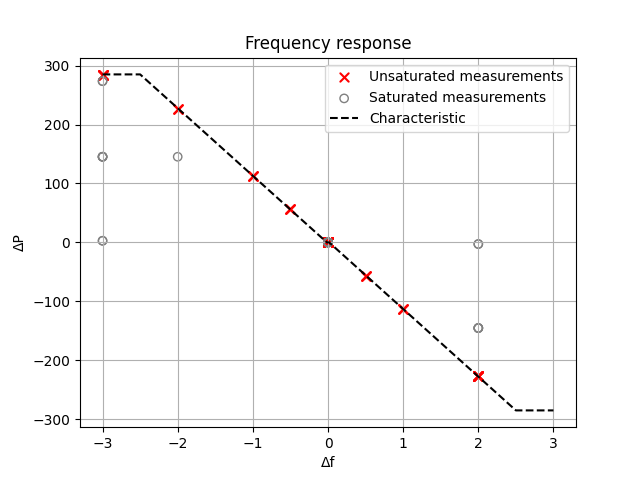
\includegraphics[width=0.7\textwidth]{\analysisdir/pscad/dpdf_characteristic.png}
		\caption{s5.2.5.11 frequency droop characteristic validation (PSCAD)}
		\label{fig:52511-frequency-droop-validation-pscad}
	\end{figure}
	
	{
		\fontsize{5}{7}\selectfont
		\autoscaledlongtable
		{s5.2.5.11 frequency droop controller test suite (PSCAD)}
		{tab:s52511-frequency-controller-test-suite-pscad}
		{\projectassetsdir/test-suite-tables/CSR/52511-Fgrid-test-table.csv}
	}

	\subsection{FCAS Results}
	The tests performed for this clause have been presented in Table \ref{tab:FCAS-test-suite} and have been provided in \ref{FCAS Tests [S5.2.5.11]}. For all tests, we see the response of the generating system aligns with the expectations outlined in \cite{aemo-fcas}.
	
	{
		\fontsize{5}{7}\selectfont
		\autoscaledlongtable
		{s5.2.5.11 FCAS test suite (PSCAD)}
		{tab:FCAS-test-suite}
		{\projectassetsdir/test-suite-tables/CSR/FCAS-test-table.csv}
	}
	
	
	
	\section{[S5.2.5.12] Impact on Network Capability}
	\subsection{Automatic Access Standard}
	\begin{tcolorbox}[lightgreenbox]
		The integrated resource system has plant capabilities and control systems that are sufficient so that when connected to the power system it does not reduce any inter-regional or intra-regional power transfer capability below the level that would apply if the integrated resource system were not connected.
	\end{tcolorbox}
	\subsection{Assessment Methodology}
	\label{sec:s52512}
	This clause is assessed through analysis of the WAN contingency test results available in the WAN studies section on page \pageref{subsubsec:WAN-results} of this report. To ensure compliance with this clause, the contingencies are applied with the generating system out of service and in service, and the results are overlayed and compared.
	
	In order to assess the impact of the project on the South Australian electrical network, four wide area cases were prepared based on recommendations provided by ElectraNet.
	
	For each case, the interconnector flows are characterised by the below.
	
	\begin{enumerate}
		\item SA light load - Interconnectors exporting 850 MW. Barker Inlet and Snapper Point in service.
		\item SA light-medium load - Interconnectors exporting 850 MW. Barker Inlet, Snapper Point, and QPS 5 in service.
		\item SA medium-high load - Interconnectors importing 750 MW. Barker Inlet, Snapper Point, Pelican unit \#1, and QPS 5 in service.
		\item SA high load - Interconnectors importing 1,300 MW. Barker Inlet, Snapper Point, Pelican units \#1 and \#2, and QPS 5 in service.
	\end{enumerate}
	
	The interconnectors and corresponding limits applicable to this project have been prepared below.
	
	\begin{table}[H]
		\centering
		\begin{tabular}{|c|c|c|}
			\hline
			Interconnector & Flow direction & Nominal Capacity (MW) \\ \hline
			Heywood (VIC-SA) & Towards VIC & 550 \\ \hline
			Heywood (VIC-SA) & Towards SA & 600 \\ \hline
			PEC (SA-VIC-NSW) & Towards NSW & 800 \\ \hline
			PEC (SA-VIC-NSW) & Towards SA & 800 \\ \hline
			Murraylink (VIC-SA) & Towards Vic & 200 \\ \hline
			Murraylink (VIC-SA) & Towards SA & 220 \\ \hline
		\end{tabular}
		\caption{Interconnector flows applicable to this project}
		\label{tab:case-interconnector-flow}
	\end{table}
	The list of faults evaluated in WAN studies was limited to those studied as part of R0 - as directed by ElectraNet.
	
	Faults were carried out using AEMO's OPDMS snapshots, which incorporated nearby generation and the generator SMIB model, and evaluated performance of the generator for disturbances on the wide area network. A variety of faults were tested, including:
	
	\begin{itemize}
		\item Three-phase-to-ground faults with circuit breaker failure clearance times
		\item Two-phase-to-ground faults
	\end{itemize}
	
	The contingencies considered for wide are network assessment are presented in Table \ref{tab:wide-area-contingencies}.
	
	\subsection{Results}
	
	
	The generating system was found not to reduce any inter-regional or intra-regional power transfer capability below the level that would apply with the generating system out of service. The results of the contingencies with the generating system in and out of service are available in Appendices \ref{WAN Case 1 - Wide Area Network Contingency Overlays [S5.2.5.12]} through \ref{WAN Case 4 - Wide Area Network Contingency Overlays [S5.2.5.12]}.
	  
	\section{[S5.2.5.13] Voltage and Reactive Power Control}
	\subsection{Automatic Access Standard}
	\begin{tcolorbox}[lightgreenbox]
		 \textbf{Voltage ‘droop’} = 4\% on 112.575 MVAr base

\begin{enumerate}
	\item The integrated resource system has plant capabilities and control systems sufficient to ensure that:
	\begin{enumerate}
		\item power system oscillations, for the frequencies of oscillation of the production unit against any other production unit or system, are adequately damped;
		\item operation of the integrated resource system does not degrade the damping of any critical mode of oscillation of the power system; and
		\item operation of the integrated resource system does not cause instability (including hunting of tap-changing transformer control systems) that would adversely impact other Registered Participants.
	\end{enumerate}
	\item The control systems used with this integrated resource system have:
	\begin{enumerate}
		\item for the purposes of disturbance monitoring and testing, permanently installed and operational, monitoring and recording facilities for key variables including each input and output; and
		\item facilities for testing the control system sufficient to establish its dynamic operational characteristics.
	\end{enumerate}
	\item The integrated resource system has facilities with a control system to regulate voltage, reactive power and power factor, with the ability to operate in any control mode and to switch between control modes, as shown in the plant voltage control strategy document
	\item The integrated resource system has a voltage control system that:
	\begin{enumerate}
		\item regulates voltage at the Connection Point to within 0.5\% of the setpoin;
		\item regulates voltage in a manner that helps to support network voltages during faults and does not prevent the NSP from achieving the requirements under clause S5.1a.3 and S5.1a.4 of the NER;
		\item allows the voltage setpoint to be continuously controllable in the range of at least 95\% to 105\% of the target voltage at [the Connection Point (as recorded in the connection agreement), without reliance on a tap-changing transformer and subject to the reactive power capability referred to in the performance standard under clause S5.2.5.1;
		\item has limiting devices to ensure that a voltage disturbance does not cause the production unit to trip at the limits of its operating capability.  The limiting devices:
			\begin{enumerate}
				\item do not detract from the performance of any power system stabiliser or power oscillation damping capability;  and
				\item are co-ordinated with all protection systems.
			\end{enumerate}
		
	\end{enumerate}
	\item The integrated resource system has a voltage control system that: 
	\begin{enumerate}
		\item with the integrated resource system connected to the power system, has settling times for active power, reactive power and voltage due to a step change of voltage setpoint or voltage at the connection point, of less than:
		\begin{enumerate}
			\item 5.0 s for a 5\% voltage disturbance with the integrated resource system connected to the power system, from an operating point where the voltage disturbance would not cause any limiting device to operate; and
			\item 7.5 s for a 5\% voltage disturbance with the integrated resource system connected to the power system, when operating into any limiting device from an operating point where a voltage disturbance of 2.5\% would just cause the limiting device to operate;
		\end{enumerate}
		\item for a 5\% step change in the voltage setpoint, has reactive power rise time, of less than 2 s;
		\item has power oscillation damping capability with sufficient flexibility to enable damping performance to be maximised with characteristics as described in paragraph (7).
	\end{enumerate}
	\item A reactive power or power factor control system provided under paragraph (3) will: 
	\begin{enumerate}
		\item regulate reactive power or power factor at the Connection Point, to within: 
		\begin{enumerate}
			\item for a integrated resource system operating in reactive power mode, 2\% of the generating system’s rating (expressed in MVAr);   
			\item for a integrated resource system operating in power factor mode, a power factor equivalent to 2\% of the integrated resource system's rating (expressed in MVAr); 
		\end{enumerate}
		\item allow the reactive power or power factor setpoint to be continuously controllable across the reactive power capability range established under the performance standard under clause S5.2.5.1; and 
		\item with the integrated resource system connected to the power system, and for a step change in setpoint of at least 50\% of the reactive power capability agreed with AEMO and the NSP under clause S5.2.5.1 of the NER, or a 5\% voltage disturbance at the location agreed under subparagraph (i):
		\begin{enumerate}
			\item have settling times for active power, reactive power and voltage of less than 5.0 s from an operating point where the voltage disturbance would not cause any limiting device to operate; and 
			\item have settling times for active power, reactive power and voltage of less than 7.5 s when operating into any limiting device from an operating point where a voltage disturbance of 2.5\% would just cause the limiting device to operate. 
		\end{enumerate}
	\end{enumerate}
\end{enumerate}

	\end{tcolorbox}
	\subsection{Assessment Methodology}
	
	Reactive controller stability tests assess the ability of the generator to provide stable reactive response to a perturbed Connection Point voltage or controller state (i.e. a reference change). In VAr and power factor control modes, this is just about  $P_{\mathrm{POC}}$ and $Q_{\mathrm{POC}}$ settling to their pre-disturbance values. However, in voltage droop control modes, a changing $V_{\mathrm{POC}}$ will result in a changing calculated $Q_{\mathrm{ref}}$, so the generator will need to track to a new reactive power target at the same time as rejecting the disturbance.

To implement these tests in \ac{SMIB} modelling, the appropriate $V_{\mathrm{grid}_{\mathrm{1}}}$
is first identified to achieve $V_{\mathrm{POC}_{\mathrm{1}}}$ given the required initial $P_{\mathrm{POC}}$, $Q_{\mathrm{POC}}$, SCR and X/R conditions. Subsequent $V_{\mathrm{grid}}$ values $V_{\mathrm{grid}_{\mathrm{2}}}, V_{\mathrm{grid}_{\mathrm{3}}}, \dots, V_{\mathrm{grid}_{\mathrm{n}}}$ can then be calculated to achieve the desired $V_{\mathrm{POC}}$ values $V_{\mathrm{POC}_{\mathrm{2}}}, V_{\mathrm{POC}_{\mathrm{3}}}, \dots, V_{\mathrm{POC}_{\mathrm{n}}}$.

With all $V_{\mathrm{grid,i}}$ calculated, a simulation is performed with $V_{\mathrm{grid}}$ stepped or ramped as required to implement the desired disturbance, as shown in Figure~\ref{fig:smib-vgrid-disturbance-diagram}.

\begin{figure}[H]
	\centering
	\newcommand{\bushere}[3]{% length, text above, text below}
% Optional arguments do nto work in paths
%
% starting point; draw an edge and then two nodes
% save the position
coordinate(tmp)
% go up and do an edge down
++(0,#1) node[anchor=base, font=\footnotesize]{#2} edge[ultra thick] ++(0, {-2*#1})
% edges do not move the current point, go down to position the node
++(0,{-2*#1}) node[below]{#3}
% go back to where we started
(tmp)
}

\ctikzset{sources/fill=gray!20, resistors/fill=gray!20}
\resizebox{\linewidth}{!}{ % Set width to \linewidth
	\begin{tikzpicture}[semithick]% default line width
		% Buses and branches
		\draw (0,0)
		node[left, font=\footnotesize]{Generator} ++(1.5,0) \bushere{1.5}{Connection Point}{} coordinate(poc);
		\draw (poc)
		-- ++ (1,0) to[generic, l={$Z_{\text{grid}}$}, resistors/width=2] ++ (4,0)
		-- ++ (1,0)
		\bushere{1.5}{Infinite Bus}{} coordinate(infinite bus);
		% One load (start from the coord load, go up)
		\ctikzset{bipoles/border margin=0.5}% See manual section 3.1.2
		\draw (infinite bus) -- ++(1,0) node[vsourcesinshape, rotate=90]{} coordinate(vgrid) ++(0.5,0) node[right]{$V_{\text{grid}}$};
		\draw (poc) -- ++(-1,0) node[vsourcesinshape, rotate=90]{};
		% Fault
		\draw[blue, font=\footnotesize, <-] (vgrid) ++(0, -0.5) -- ++(0, -0.5) -- ++(0.5,0) node[right]{$V_{\mathrm{grid}_{\mathrm{1}}}, V_{\mathrm{grid}_{\mathrm{2}}}, V_{\mathrm{grid}_{\mathrm{3}}}, \dots, V_{\mathrm{grid}_{\mathrm{n}}}$};
		
	\end{tikzpicture}
}






	\caption{Reactive power controller disturbance assessment methodology}
	\label{fig:smib-vgrid-disturbance-diagram}
\end{figure}

To assess the stability of the control system response to a stepped $V_{\mathrm{ref}}$, $Q_{\mathrm{ref}}$, $PF_{\mathrm{ref}}$ signal, reference steps are applied as per Figure \ref{fig:smib-vref-change-diagram}. To perform this test, the generator is first initialised to the initial $V_{\mathrm{POC}}$, $P_{\mathrm{POC}}$, $Q_{\mathrm{POC}}$, SCR and X/R conditions, where $Q_{\mathrm{POC}}$ is the target reactive output of the generator for the associated $V_{\mathrm{err}} = V_{\mathrm{ref}_{\mathrm{1}}} - V_{\mathrm{POC}}$ per the droop characteristic.

Once the generator has been initialised, the series of voltage references $V_{\mathrm{ref}_{\mathrm{2}}}, V_{\mathrm{ref}_{\mathrm{3}}}, \dots, V_{\mathrm{ref}_{\mathrm{n}}}$ are applied to the PPC, as shown in Figure~\ref{fig:smib-vref-change-diagram}. Tests where the reactive power reference is constrained by a reactive power limit, will be identified as "Saturating".

\begin{figure}[H]
	\centering
	\newcommand{\bushere}[3]{% length, text above, text below}
% Optional arguments do nto work in paths
%
% starting point; draw an edge and then two nodes
% save the position
coordinate(tmp)
% go up and do an edge down
++(0,#1) node[anchor=base, font=\footnotesize]{#2} edge[ultra thick] ++(0, {-2*#1})
% edges do not move the current point, go down to position the node
++(0,{-2*#1}) node[below]{#3}
% go back to where we started
(tmp)
}

\ctikzset{sources/fill=gray!20, resistors/fill=gray!20}
\resizebox{\linewidth}{!}{ % Set width to \linewidth
	\begin{tikzpicture}[semithick]% default line width
		% Buses and branches
		\draw (0,0)
		node[left, font=\footnotesize]{Generator} ++(1.5,0) \bushere{1.5}{Connection Point}{} coordinate(poc);
		\draw (poc)
		-- ++ (1,0) to[generic, l={$Z_{\text{grid}}$}, resistors/width=2] ++ (4,0)
		-- ++ (1,0)
		\bushere{1.5}{Infinite Bus}{} coordinate(infinite bus);
		% One load (start from the coord load, go up)
		\ctikzset{bipoles/border margin=0.5}% See manual section 3.1.2
		\draw (infinite bus) -- ++(1,0) node[vsourcesinshape, rotate=90]{} coordinate(vgrid) ++(0.5,0) node[right]{$V_{\text{grid}}$};
		\draw (poc) -- ++(-1,0) node[vsourcesinshape, rotate=90]{} coordinate(generator);
		% Fault
		\draw[blue, font=\footnotesize, <-] (generator) ++(0, -0.5) -- ++(0, -0.5) -- ++(-0.5,0) node[left]{$V_{\mathrm{ref}_{\mathrm{1}}}, V_{\mathrm{ref}_{\mathrm{2}}}, V_{\mathrm{ref}_{\mathrm{3}}}, \dots, V_{\mathrm{ref}_{\mathrm{n}}}$};
		
	\end{tikzpicture}
}






	\caption{Reactive power controller disturbance assessment methodology (shown for voltage droop control)}
	\label{fig:smib-vref-change-diagram}
\end{figure}

In wide area studies, only reference step tests are applied, since actual voltage disturbances are best assessed through the application of real faults, machine trips and \ac{TOV} shunt application, all of which is assessed under s5.2.5.5.


	
	All SMIB assessments for this clause have been performed in PSCAD and all wide-area assessments have been performed in PSS/E. All tests undertaken as part of this clause have been characterised as either "Saturated" or "Un-saturated". Saturating tests are those for which the reference step is limited by the reactive power controller. Unsaturated tests are those for which the reference step stays within the reactive power limits of the reactive power controller. Please note that as the voltage droop configured for this plant is 2\% on a base of 23.7 MVAr, all voltage steps applied result in operation of the reactive power controllers limits. 
	
	\subsection{SMIB study results}
	
	\subsubsection{Oscillation Rejection}
	Oscillation rejection analysis has been performed to ensure that the generating system acts to adequately damp oscillations seen at the connection point in accordance with section (1) of this GPS clause. Please refer to the results in Appendix \ref{Grid oscillation rejection tests [S5.2.5.13]} which demonstrate the generators response to oscillations of varying frequency.
	
	\subsubsection{Connection point voltage disturbance tests (droop mode)}
	\label{subsec:s52513-vgrid-steps-droop-mode}
	
	The connection point voltage disturbance tests performed for this clause have been presented in Table \ref{tab:s52513-vgrid-droop-step-table}. Figure \ref{fig:s52513-vgrid-droop-saturated-step-summary-plot} shows the active power, reactive power and connection point voltages along with the distribution of rise and settling times (as applicable). The results show compliance to the GPS requirements for all tests.
	
	Figure \ref{fig:s52513-vdroop-controller-accuracy} presents a summary of all $Q_{\mathrm{POC}}$ measurements against $V_{\mathrm{POC}}$ measurements at the end of each connection point voltage disturbance tests after the controllers have settled. It can be seen from this chart that the controller always accurately regulates to the intended voltage droop characteristic.
	
	
	\begin{figure}[H]
		\centering
		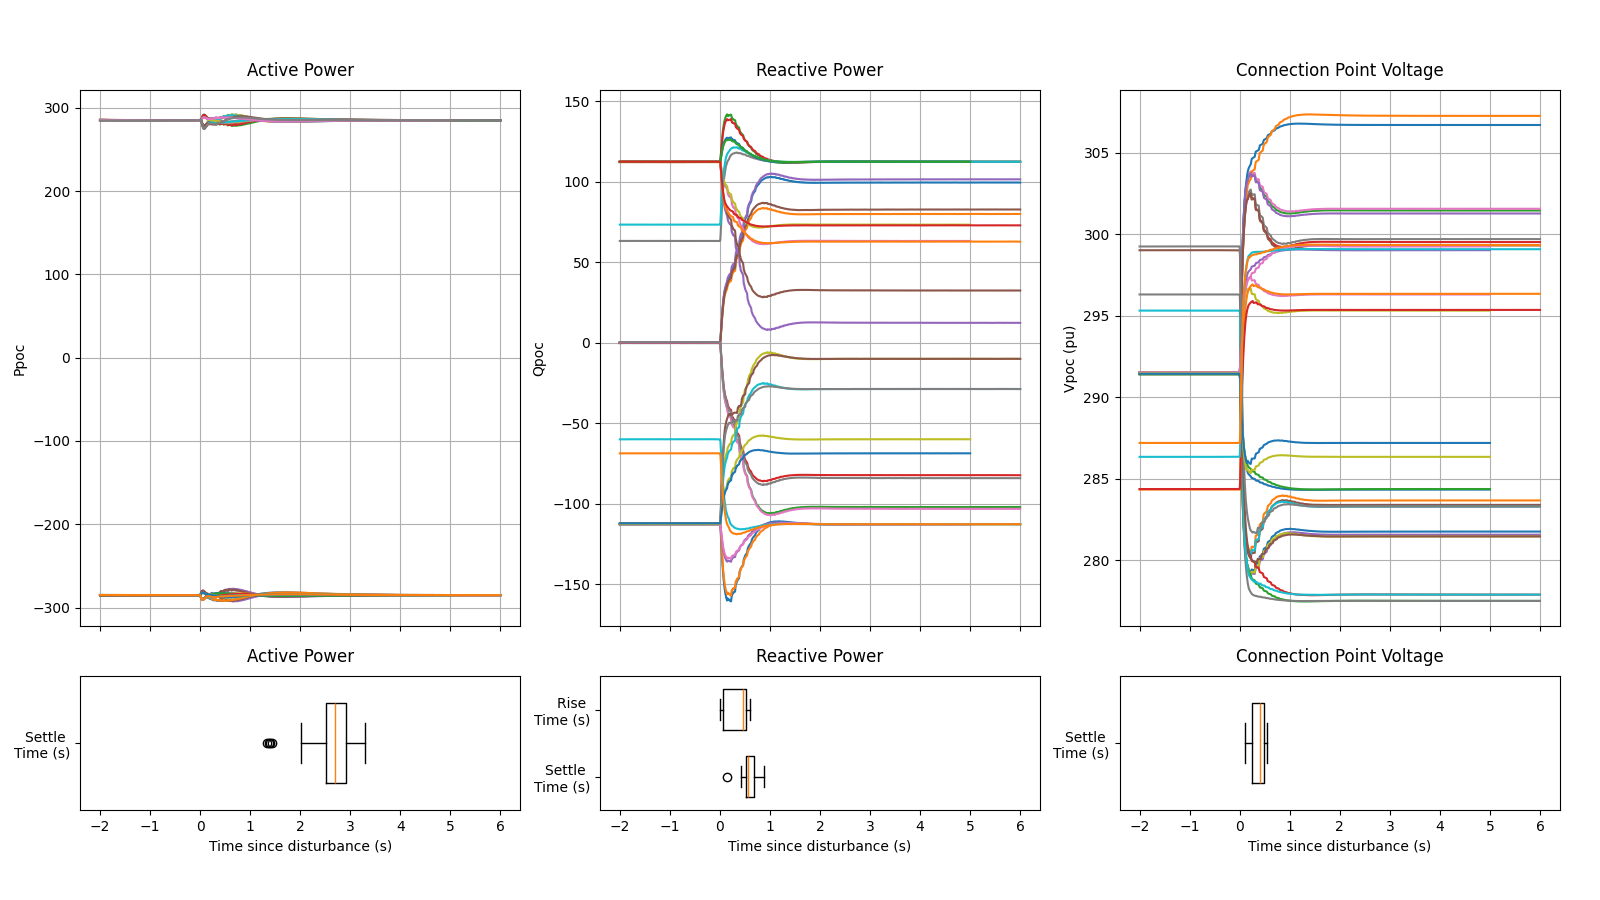
\includegraphics[width=0.9\textwidth]{\analysisdir/pscad/Vgrid droop step disturbance tracking saturated.png}
		\caption{s5.2.5.13 Connection point voltage disturbance step test performance summary (droop mode)}
		\label{fig:s52513-vgrid-droop-saturated-step-summary-plot}
	\end{figure}
	
	\begin{figure}[H]
		\centering
		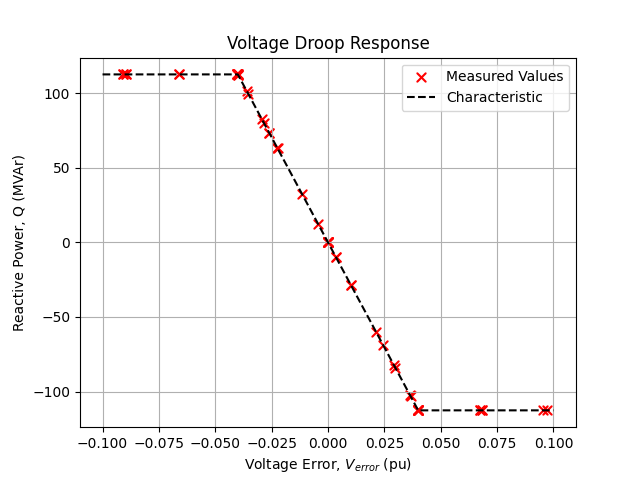
\includegraphics[width=0.7\textwidth]{\analysisdir/pscad/vdroop_characteristic.png}
		\caption{Voltage droop controller characteristic accuracy}
		\label{fig:s52513-vdroop-controller-accuracy}
	\end{figure}
	
	{
		\fontsize{7}{8}\selectfont
		\autoscaledlongtable
		{s5.2.5.13 Connection point voltage disturbance step test suite (droop mode)}
		{tab:s52513-vgrid-droop-step-table}
		{\projectassetsdir/test-suite-tables/CSR/52513-Vgrid-droop-test-table.csv}
	}

	Table \ref{tab:s52513-vgrid-droop-step-results-table} shows the rise and settling times for each test performed. Please note that tests 9-12 are limiter tests, while tests 1 through 8 are non-limiter tests. As seen from the table below the generating system has settling time for reactive power and voltage of less than 5.0s for all cases considered. Please note that active power settle time has not been assessed for any tests in which the change in active power is $\leq$ 0.1pu. Reactive power rise time remains below 2 seconds for all non-limiter tests.
	
	{
		\fontsize{6.5}{11}\selectfont
		\autoscaledlongtable
		{s5.2.5.13 Voltage grid disturbance step test results (droop mode)}
		{tab:s52513-vgrid-droop-step-results-table}
		{report-assets/analysis/pscad/Vgrid droop step disturbance tracking saturated.csv}
	}
	
	
	\subsubsection{Voltage reference step tests}
	
	The connection point voltage reference step tests performed for this clause have been presented in Table \ref{tab:s52513-vref-step-table}. Figure \ref{fig:s52513-vref-step-saturated-summary-plot} shows the active power, reactive power and connection point voltages along with the distribution of rise and settling times (as applicable) The results show compliance to the GPS requirements for all tests.
	
	
	\begin{figure}[H]
		\centering
		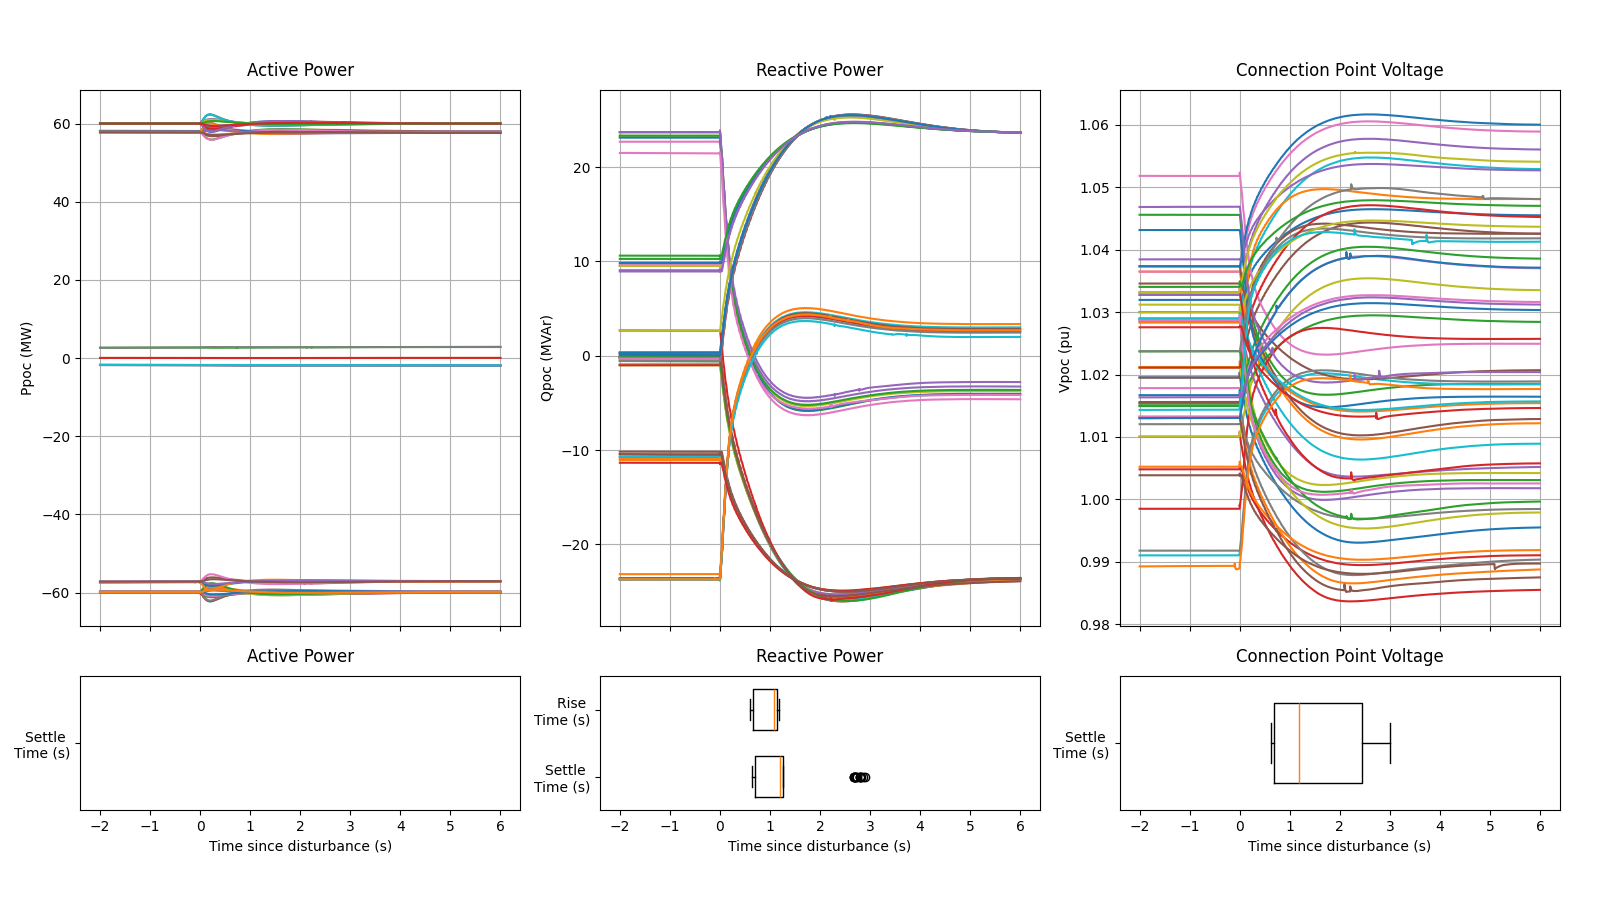
\includegraphics[width=0.9\textwidth]{\analysisdir/pscad/Vref step disturbance tracking saturated.png}
		\caption{s5.2.5.13 Voltage reference step test performance summary}
		\label{fig:s52513-vref-step-saturated-summary-plot}
	\end{figure}
	
	{
		\fontsize{9}{8}\selectfont
		\autoscaledlongtable
		{s5.2.5.13 Voltage reference step test suite}
		{tab:s52513-vref-step-table}
		{\projectassetsdir/test-suite-tables/CSR/52513-Vref-test-table.csv}
	}

	Table \ref{tab:s52513-vref-step-results-table} shows the rise and settling times for each test performed. Please note that active power settling times were not assessed as the change in active power was found to be $\leq$ 0.1 pu for all tests performed.
	
	{
		\fontsize{6.5}{11}\selectfont
		\autoscaledlongtable
		{s5.2.5.13 Voltage reference step test results}
		{tab:s52513-vref-step-results-table}
		{report-assets/analysis/pscad/Vref step disturbance tracking saturated.csv}
	}
	
	\subsubsection{Reactive power reference step tests}
	
	The connection point reactive power reference step tests performed for this clause have been presented in Table \ref{tab:s52513-qref-step-table}. Figure \ref{fig:s52513-qref-step-saturated-summary-plot} shows the active power, reactive power and connection point voltages along with the distribution of rise and settling times (as applicable). The results show compliance to the GPS requirements for all tests.
	
	
	\begin{figure}[H]
		\centering
		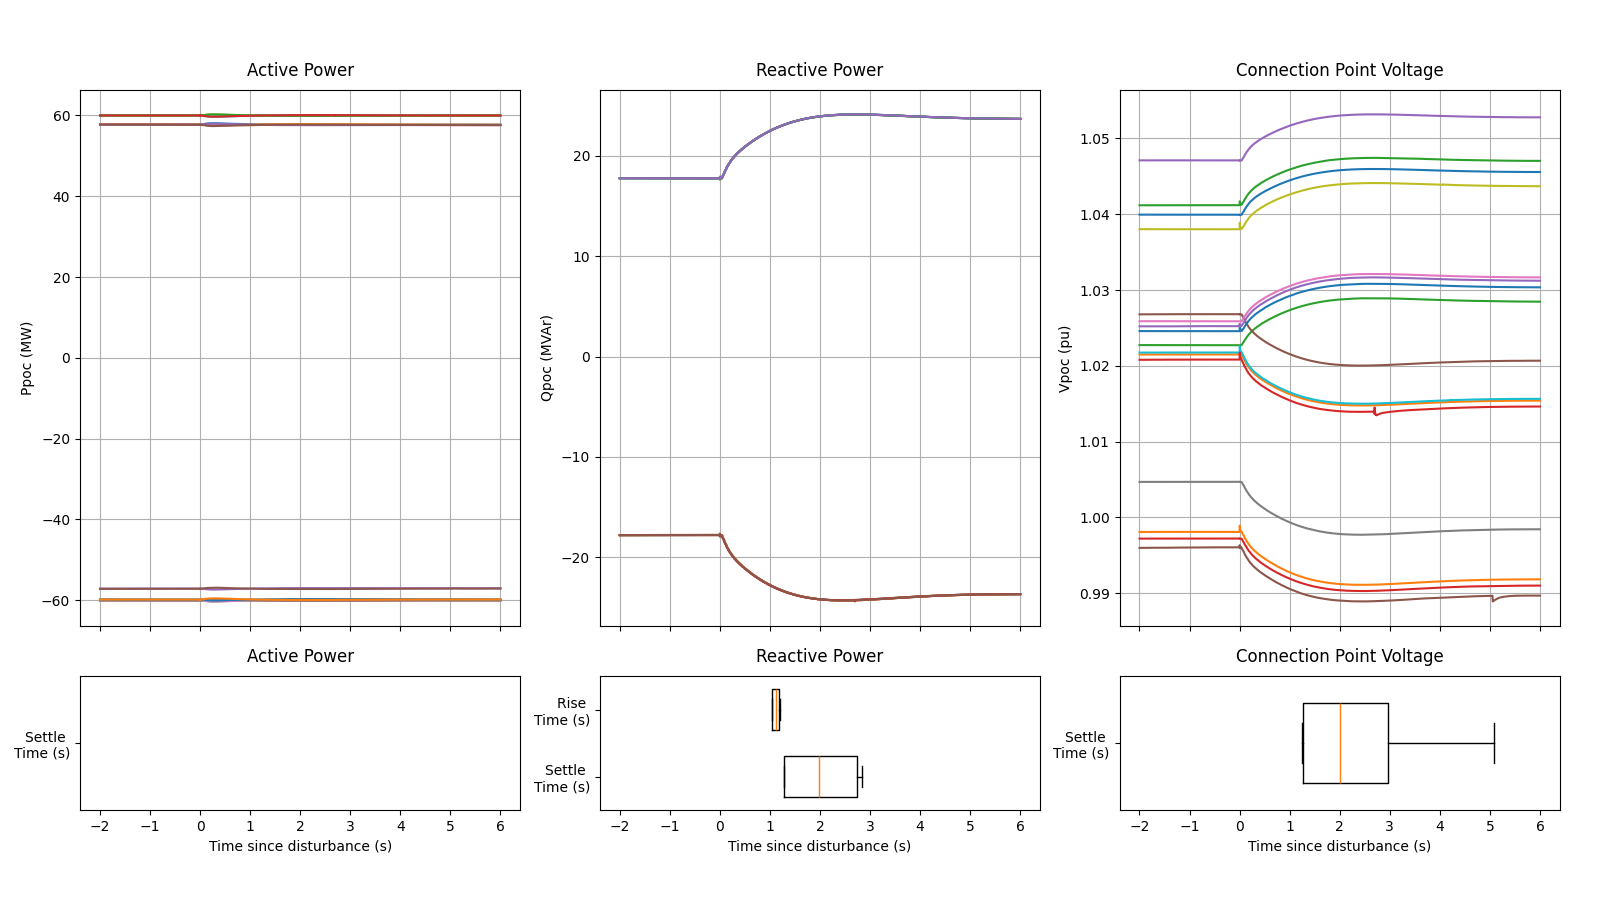
\includegraphics[width=0.9\textwidth]{\analysisdir/pscad/Qref step disturbance tracking saturated.png}
		\caption{s5.2.5.13 VAr reference step test performance summary}
		\label{fig:s52513-qref-step-saturated-summary-plot}
	\end{figure}
	

	
	{
		\fontsize{7}{9}\selectfont
		\autoscaledlongtable
		{s5.2.5.13 VAr reference step test suite}
		{tab:s52513-qref-step-table}
		{\projectassetsdir/test-suite-tables/CSR/52513-Qref-test-table.csv}
	}

	
	Table \ref{tab:s52513-qref-step-results-table-sat} shows the rise and settling times for each test performed. Please note that active power settling time was not assessed for this clause as the change in active power for all tests was negligible. The table below demonstrates compliance for all reactive power reference steps performed.
	
	{
		\fontsize{6.5}{9}\selectfont
			\autoscaledlongtable%
			{s5.2.5.13 VAr reference step test results (saturated)}%
			{tab:s52513-qref-step-results-table-sat}%
			{report-assets/analysis/pscad/Qref step disturbance tracking saturated.csv}%
	}
	

	
	\subsubsection{Power factor reference step tests}
	
	The connection point power factor power reference step tests performed for this clause have been presented in Table \ref{tab:s52513-pfref-step-table}. Figure  \ref{fig:s52513-pfref-step-saturated-summary-plot} shows the active power, reactive power and connection point voltages along with the distribution of rise and settling times (as applicable). The results show compliance to the GPS for all tests.
	
	\begin{figure}[H]
		\centering
		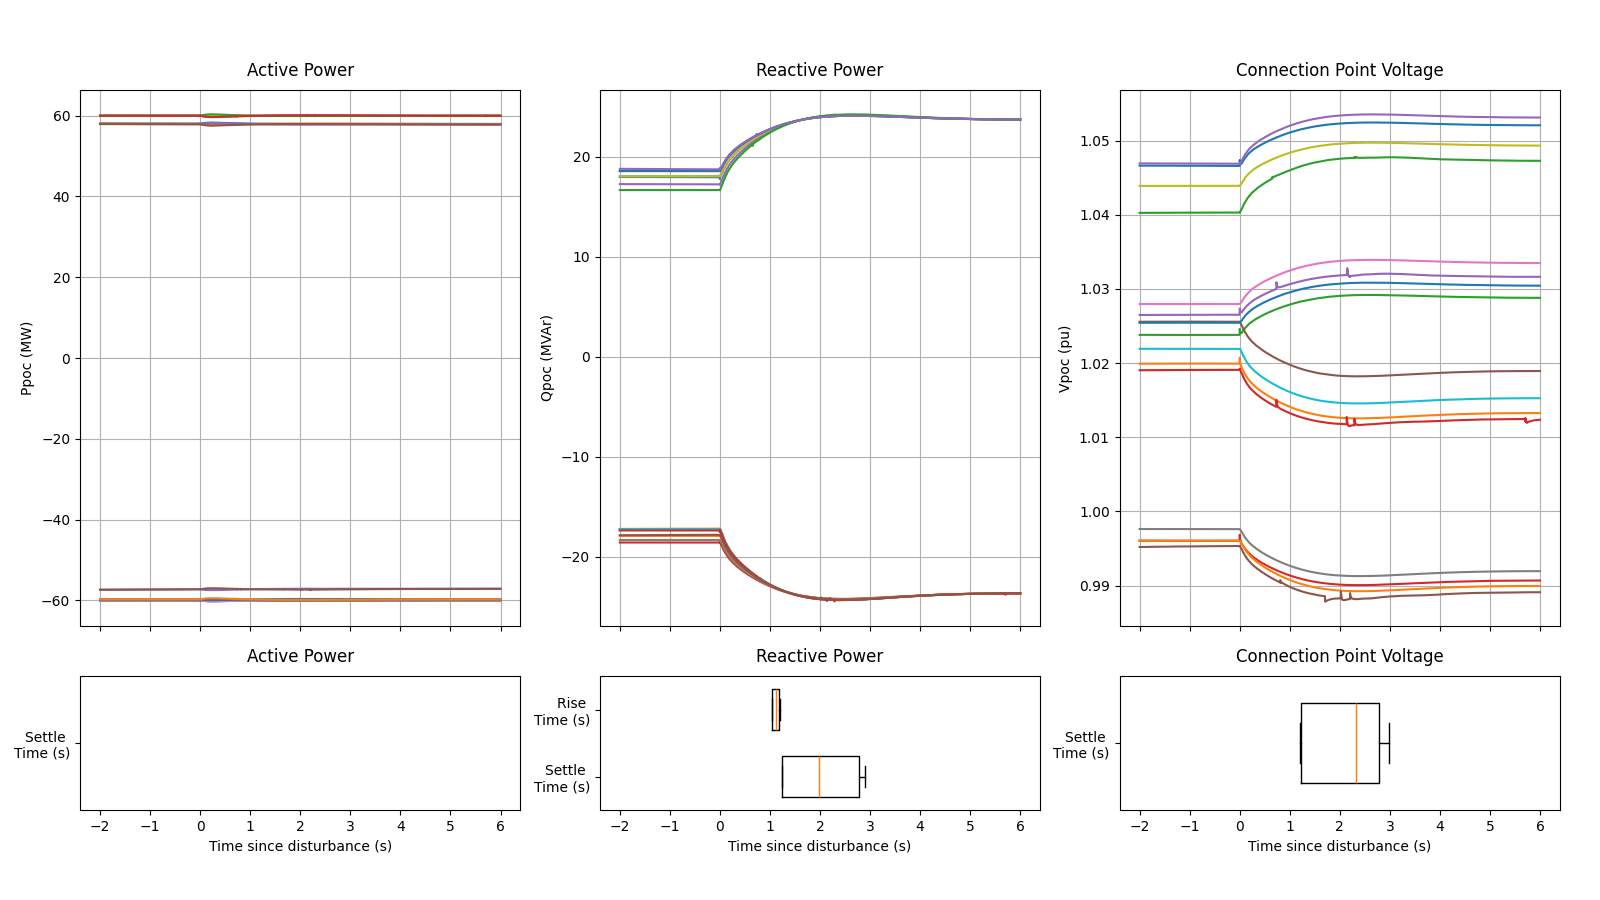
\includegraphics[width=0.9\textwidth]{\analysisdir/pscad/PFref step disturbance tracking saturated.png}
		\caption{s5.2.5.13 PF reference step test performance summary}
		\label{fig:s52513-pfref-step-saturated-summary-plot}
	\end{figure}
	

	
	{
		\fontsize{6}{8}\selectfont
		\autoscaledlongtable
		{s5.2.5.13 PF reference step test suite}
		{tab:s52513-pfref-step-table}
		{\projectassetsdir/test-suite-tables/CSR/52513-PFref-test-table.csv}
	}

	
	Table \ref{tab:s52513-pfref-step-results-table} shows the rise and settling times for each test performed. The results below show compliance to the GPS for all tests.
	
	
	{
		\fontsize{6.5}{9}\selectfont
		\autoscaledlongtable
		{s5.2.5.13 PF reference step test results}
		{tab:s52513-pfref-step-results-table}
		{report-assets/analysis/pscad/PFref step disturbance tracking saturated.csv}
	}
	
	\subsection{Wide area study results}
	
	\subsubsection{Voltage reference step tests}
	
	
	The connection point voltage reference step tests performed in the wide area PSSE network have been presented in Table \ref{tab:wan-s52513-vref-step-table}. Please note that active power settle times were not assessed for these tests as the change in active power was found to be negligible. The results show compliance to the GPS requirements for all tests.	
	


	
	{
		\fontsize{6}{8}\selectfont
		\autoscaledlongtable
		{s5.2.5.13 Voltage reference step test suite}
		{tab:wan-s52513-vref-step-table}
		{\projectassetsdir/test-suite-tables/PSSE-WAN/52513-Vref-test-table.csv}
	}
	

	
	\subsubsection{Reactive power reference step tests}
	
	The connection point reactive power reference step tests performed in the wide area PSSE network have been presented in Table \ref{tab:wan-s52513-qref-step-table}. Please note that active power settle times were not assessed for these tests as the change in active power was found to be negligible.The results show compliance to the GPS requirements for all tests.




	
	{
		\fontsize{6}{8}\selectfont
		\autoscaledlongtable
		{s5.2.5.13 Reactive power reference step test suite}
		{tab:wan-s52513-qref-step-table}
		{\projectassetsdir/test-suite-tables/PSSE-WAN/52513-Qref-test-table.csv}
	}



	
	\subsubsection{Power factor reference step tests}
	
	The connection point power factor reference step tests performed in the wide area PSSE network have been presented in Table \ref{tab:wan-s52513-pfref-step-table}. Please note that active power settle times were not assessed for these tests as the change in active power was found to be negligible. The results show compliance to the GPS requirements for all tests.
	

	
	{
		\fontsize{6}{8}\selectfont
		\autoscaledlongtable
		{s5.2.5.13 Power factor reference step test suite}
		{tab:wan-s52513-pfref-step-table}
		{\projectassetsdir/test-suite-tables/PSSE-WAN/52513-PFref-test-table.csv}
	}
	

	
	
	\section{[S5.2.5.14] Active Power Control}
	\subsection{Automatic Access Standard}
	\begin{tcolorbox}[lightgreenbox]
		The integrated resource system has an active power control system that is adequately damped and capable of:
\begin{enumerate}
	\item maintaining and changing its active power level in accordance with its dispatch instructions; 
	\item ramping its active power level linearly from one dispatch level to another; and
	\item receiving and automatically responding to signals delivered from the automatic generation control system, as updated at a rate of once every 4 s  
\end{enumerate}

	\end{tcolorbox}
	\subsection{Assessment Methodology}
	
	Active power reference step tests assess the ability of the generator to provide a damped active (and reactive) power response to a change in the active power target applied to the PPC.

To perform this test, the generator is first initialised to the initial $V_{\mathrm{POC}}$, $P_{\mathrm{POC}}$, $Q_{\mathrm{POC}}$, SCR and X/R conditions, where $P_{\mathrm{POC}} = P_{\mathrm{ref}_{\mathrm{1}}}$. Once the generator has been initialised, the series of active power references $P_{\mathrm{ref}_{\mathrm{2}}}, P_{\mathrm{ref}_{\mathrm{3}}} \dots, P_{\mathrm{ref}_{\mathrm{n}}}$ are applied to the PPC, as shown in Figure~\ref{fig:smib-pref-change-methodology}.

\begin{figure}[h]
	\centering
	\newcommand{\bushere}[3]{% length, text above, text below}
% Optional arguments do nto work in paths
%
% starting point; draw an edge and then two nodes
% save the position
coordinate(tmp)
% go up and do an edge down
++(0,#1) node[anchor=base, font=\footnotesize]{#2} edge[ultra thick] ++(0, {-2*#1})
% edges do not move the current point, go down to position the node
++(0,{-2*#1}) node[below]{#3}
% go back to where we started
(tmp)
}

\ctikzset{sources/fill=gray!20, resistors/fill=gray!20}
\resizebox{\linewidth}{!}{ % Set width to \linewidth
	\begin{tikzpicture}[semithick]% default line width
		% Buses and branches
		\draw (0,0)
		node[left, font=\footnotesize]{Generator} ++(1.5,0) \bushere{1.5}{Connection Point}{} coordinate(poc);
		\draw (poc)
		-- ++ (1,0) to[generic, l={$Z_{\text{grid}}$}, resistors/width=2] ++ (4,0)
		-- ++ (1,0)
		\bushere{1.5}{Infinite Bus}{} coordinate(infinite bus);
		% One load (start from the coord load, go up)
		\ctikzset{bipoles/border margin=0.5}% See manual section 3.1.2
		\draw (infinite bus) -- ++(1,0) node[vsourcesinshape, rotate=90]{} coordinate(vgrid) ++(0.5,0) node[right]{$V_{\text{grid}}$};
		\draw (poc) -- ++(-1,0) node[vsourcesinshape, rotate=90]{} coordinate(generator);
		% Fault
		\draw[blue, font=\footnotesize, <-] (generator) ++(0, -0.5) -- ++(0, -0.5) -- ++(-0.5,0) node[left]{$P_{\mathrm{ref}_{\mathrm{1}}}, P_{\mathrm{ref}_{\mathrm{2}}}, P_{\mathrm{ref}_{\mathrm{3}}}, \dots, P_{\mathrm{ref}_{\mathrm{n}}}$};
		
	\end{tikzpicture}
}






	\caption{Active power reference change methodology}
	\label{fig:smib-pref-change-methodology}
\end{figure}
	
	All assessments for this clause have been performed in PSCAD.
	
	\subsection{Results}
	
	The full suite of active power control tests are shown in Table \ref{tab:s52514-test-suite}. The results demonstrate that the generating system is capable of ramping stably without a defined ramp rate limit.The tests provided here demonstrate the ability for the generator to ramp linearly from setpoint to the next over a five minute interval.
	
	\begin{table}[H]
		\centering
		\caption{s5.2.5.14 active power control test suite}
		\label{tab:s52514-test-suite}
		\autoscaledtable{H}{\projectassetsdir/test-suite-tables/CSR/52514-Pref-test-table.csv}
	\end{table}


	\section{[S5.2.8 and S5.3.2(b)] Fault Current}
	\subsection{Agreed Access Standard}	
	\begin{tcolorbox}[lightgreenbox]
		\begin{itemize}
	\item The generating system limits its contribution to the fault current at the Connection Point to:
	\begin{itemize}
		\item Three-phase fault current: 1.57 kA;
		\item Single-phase-to-ground fault current: 4.7 kA;
		\item Phase-to-phase-to-ground fault current: 2.71 kA.
	\end{itemize}
	\item The generating system’s connected plant is capable of withstanding fault current through the connection point up to 40 kA for 1000 ms.
	\item The circuit breaker provided to isolate the generating system from the network is capable of breaking, without damage or restrike, the maximum fault current of 40 kA, expected to flow through the circuit breaker for any fault in the network or in the generating system.
\end{itemize}

	\end{tcolorbox}

	\subsection{Assessment Methodology}
	As the vector group of the main transformer for this generating system is a wye-wye configuration with grounded neutrals, the only path for zero-sequence current to flow will be provided by the grid beyond the generators point of connection. A consequence of this is that the generators fault current contribution for earth faults will be dominated by the zero-sequence impedance seen by the POC.
	
	In order to estimate a likely fault current contribution, the ASCC fault current simulation method was used in the PSS/E low and high load wide area network models to determine the three-phase-to-ground, single-phase-to-ground, and phase-to-phase-to-ground fault current contribution at the generating system's POC at a voltage of 1.0 pu. 
	
	In order to estimate an upper-bound on the generating systems fault current contribution the ASCC fault current simulation method was utilised in the SMIB model. For this assessment, the zero-sequence reactance of the grid impedance was reduced to 0.00001 pu.
		
	In assessing the plants withstand capability, please refer to the protection study report which includes a summary of the maximum and minimum expected fault levels as well as equipment ratings \cite{protection-design-report}.
	
	\subsection{Results}
	An estimate of the likely maximum fault current contribution by fault type - based on the wide area network grid impedances seen by the generating system, have been prepared in Table \ref{tab:528-results}.

	\begin{table}[H]
	\centering
	\caption{Approximate Fault current contribution (WAN)}
	\label{tab:528-results}
	\begin{tabular}{|l|c|c|c|}
		\hline
		\textbf{Case} & \textbf{3phg}  & \textbf{1phg} & \textbf{ph-phg} \\
		\hline
		Case 1 - Low Load & 0.450 kA   & 0.224 kA & 0.378 kA\\
		\hline
		Case 4 - High Load & 0.450 kA  & 0.223 kA & 0.378 kA\\
		\hline
	\end{tabular}			
	\end{table}
	
	An estimate of the upper-bound on the maximum fault current contribution calculated for each type of fault is shown in Table \ref{tab:528-results-upperbound}.

	\begin{table}[H]
		\centering
		\caption{Upper-bound on fault current contribution (SMIB)}
		\label{tab:528-results-upperbound}
		\begin{tabular}{|l|c|c|}
			\hline
			\textbf{Fault Type} & \textbf{1.0pu voltage}  & \textbf{1.1pu voltage} \\
			\hline
			Three-phase fault 				& 0.450 kA 	& 0.496 kA \\
			\hline
			Single phase-to-ground fault 	& 0.416 kA 	& 0.457 kA  \\
			\hline
			Phase-to-phase-to-ground fault 	& 0.440 kA	&  0.484 kA \\
			\hline
		\end{tabular}			
	\end{table}

	From the above analysis we see that the 3phg, 1Ph-g,and 1Ph-Ph-G fault current contribution exceeds that specified in the existing Generator Performance Standard. As such we would recommend that the Generator Performance Standard is revised to align with fault contributions set to at least those reflected in Table \ref{tab:528-results-upperbound}.
	
	\section{ESCOSA License Conditions}	
	Assessment of compliance to the ESCOSA model license conditions \cite{escosa} has been undertaken in the sections below.
	
	\subsection{Disturbance Ride Through Capability}
	\begin{tcolorbox}[lightgreenbox]
		The generating system must not include any vector shift or similar relay/protective function acting upon voltage phase angle which might operate for phase angle changes less than 20 degrees.


	\end{tcolorbox}
	Compliance to this clause has been ensured as part of R1 detailed design. Please refer to the Protection Setting Report \cite{protection-design-report} which outlines protection functions for this generating system. Additionally, SMA has confirmed that the SCS3600 UP inverters do not trip on asymmetrical phase currents, voltage or angles - there is no such relay to facilitate this. As such the inverters are able to ride-through significant vector jumps. Please also refer to the SMA NER Compliance Report \cite{SMA-NER-compliance-report}.
	\subsection{System Strength}
	\begin{tcolorbox}[lightgreenbox]
		Individual components of plant within a generating system, which includes but is not limited to generating units and dynamic reactive power plant, must be capable of operating down to the following levels at the high voltage terminals in relation to each component:

\begin{enumerate}[label=(\alph*)]
	\item minimum short circuit ratio of 1.5, and  
	\item minimum positive sequence X/R ratio of 2  
\end{enumerate}
	\end{tcolorbox}
	Please refer to the provided SMA technical note on Sunny Central (Storage) UP Operation at low SCR \cite{low-scr}. This note confirms the ability of the inverters to maintain stable operation at SCRs as low as 1.0. SMA has separately confirmed that "there are no further limitations from an X/R perspective".


	
	
	\chapter*{Acronyms}
\begin{acronym}%[JSONP]\itemsep0pt
	\acro{AAS}{Automatic Access Standard}
	\acro{AEMO}{Australian Energy Market Operator}
	\acro{VSL}{Voltage Stackable Logic}
	\acro{AGC}{Automatic Generation Control}
	\acro{AVR}{Automatic Voltage Regulator}
	\acro{BESS}{Battery Energy Storage System}
	\acro{BOP}{Balance Of Plant}
	\acro{CGBESS}{Clements Gap BESS}
	\acro{Heywood BESS}{Heywood Battery Energy Storage System}	
	\acro{CSR}{Connection Studies Report}
	\acro{CT}{Current Transformer}
	\acro{CUO}{Continuous Uninterrupted Operation}
	\acro{HV}{High Voltage}
	\acro{DMAT}{Dynamic Model Acceptance Test}
	\acro{DYR}{PSSE Dynamics Data File}
	\acro{EMT}{Electromagnetic Transients}
	\acro{FIA}{Full Impact Assessment}
	\acro{FRT}{Fault Ride-Through}
	\acro{GPS}{Generator Performance Standards}
	\acro{HVRT}{High Voltage Ride-Through}
	\acro{LV}{Low Voltage}
	\acro{LVRT}{Low Voltage Ride-Through}
	\acro{MV}{Medium Voltage}
	\acro{NEM}{National Electricity Market}
	\acro{NSP}{Network Service Provider}
	\acro{OEM}{Original Equipment Manufacturer}
	\acro{OFRT}{Over-Frequency Ride-Through}
	\acro{OLTC}{On-Load Tap Changer}
	\acro{OPDMS}{Operations and Planning Data Management System}
	\acro{OVRT}{Over-Voltage Ride-Through}
	\acro{PLL}{Phase-Locked Loop}
	\acro{PLR}{Partial Load Rejection}
	\acro{PPC}{Power Plant Controller}
	\acro{PPM}{Power Plant Manager}
	\acro{RoCoF}{Rate of Change of Frequency}
	\acro{RMS}{Root Mean Square}
	\acro{RMU}{Ring Main Unit}
	\acro{RUG}{Releasable User Guide}
	\acro{S5251}{Reactive Power Capability}
	\acro{S5254}{Generating System Response to Voltage Disturbances}
	\acro{SCR}{Short Circuit Ratio}
	\acro{SMIB}{Single Machine, Infinite Bus}
	\acro{SLD}{Single Line Diagram}
	\acro{TOV}{Temporary Over-Voltage}
	\acro{UFRT}{Under-Frequency Ride-Through}
	\acro{UVRT}{Under-Voltage Ride-Through}
	\acro{VCS}{Voltage Control Strategy}
	\acro{WAN}{Wide Area Network}
	\acro{WF}{Wind Farm}
	\acro{VOIP}{Voice Over Internet Protocol}
	\acro{VRR}{Voltage Regulation Relay}
	\acro{VT}{Voltage Transformer}
\end{acronym}
	\renewcommand\bibname{References}

\begin{thebibliography}{99}	
	\bibitem{mvps-sld}MVPS SLD\\
	(PSD1834-110-001-002.pdf)
	\bibitem{mvt-datasheet}Medium Voltage Transformer Datasheet\\
	(CG_D_00181175_03_General MVT Datasheet.pdf.pdf)
	\bibitem{main-tx-datasheet} Main Transformer Datasheet\\
	(Main Transformer Datasheet.pdf)
	\bibitem{substation-sld} Substation SLD\\
	(PSD1834-110-001-001.pdf)
	\bibitem{avr-manual}TAPCON 230 AVR manual\\
	(bal_3552133_02_001_1_en.pdf)
	\bibitem{oltc-switching} OLTC Switching Datasheet\\
	(VACUTAP®_VV®_Operating_Instructions.pdf)
	\bibitem{harmonic-assessment} Harmonic Emmissions Report\\
	(PSD1834-100-100---Harmonic-Emissions-Assessment-and-Filter-Design-Rev-B.pdf)
	\bibitem{scada-philo} SCADA Control Philosophy\\
	(PSD1834-200-009---SCADA-CONTROL-PHILOSOPHY-Rev.3.pdf)
	\bibitem{aemo-io} AEMO IO Schedule\\
	(PSD1834-200-005-AEMO IO SCHEDULE-REV-04.pdf)
	\bibitem{comms-arch} Communication Architecture\\
	(PSD1834-210-003-001---COMMUNICATION-ARCHITECTURE-Rev.1.pdf)
	\bibitem{scada-spec} SCADA Functional Specification\\
	(PSD1834-200-001 - SCADA SYSTEM FUNCTIONAL DESIGN SPECIFICATION Rev.4.pdf)
	\bibitem{protection-settings-report} Protection Settings Report\\
	(PSD1834-100-007---CGBESS-Protection-Setting-Report---REV-C.pdf)



\end{thebibliography}
	
	\chapter{Appendices}
	\renewcommand{\thesection}{%
		\AlphAlph{\value{section}}%
	}

	\section{Grid Frequency Disturbance Withstand Tests [S5.2.5.3]}
	\label{Grid Frequency Disturbance Withstand Tests [S5.2.5.3]}
	
	\section{Grid Voltage Disturbance Withstand Tests [S5.2.5.4]}
	\label{Grid Voltage Disturbance Withstand Tests [S5.2.5.4]}
	
	\section{Continuous Uninterrupted Operation [S5.2.5.4]}
	\label{Continuous Uninterrupted Operation [S5.2.5.4]}
	
	\section{Balanced Faults [S5.2.5.5]}
	\label{Balanced Faults [S5.2.5.5]}
	
	\section{Unbalanced Faults [S5.2.5.5]}
	\label{Unbalanced Faults [S5.2.5.5]}
	
	\section{Temporary Over-Voltage Tests [S5.2.5.5]}
	\label{Temporary Over-Voltage Tests [S5.2.5.5]}
	
	\section{WAN Case 1 - Wide Area Network Contingency 
		\\
		Results [S5.2.5.5]}
	\label{WAN Case 1 - Wide Area Network Contingency Results [S5.2.5.5]}
	
	\section{WAN Case 2 - Wide Area Network Contingency 
		\\
		Results [S5.2.5.5]}
	\label{WAN Case 2 - Wide Area Network Contingency Results [S5.2.5.5]}
	
	\section{WAN Case 3 - Wide Area Network Contingency 
		\\
		Results [S5.2.5.5]}
	\label{WAN Case 3 - Wide Area Network Contingency Results [S5.2.5.5]}
	
	\section{WAN Case 4 - Wide Area Network Contingency 
		\\
		Results [S5.2.5.5]}
	\label{WAN Case 4 - Wide Area Network Contingency Results [S5.2.5.5]}
	
	\section{Partial Load Rejection Tests [S5.2.5.7]}
	\label{Partial Load Rejection Tests [S5.2.5.7]}
	
	\section{Frequency Protection Tests [S5.2.5.8]}
	\label{Frequency Protection Tests [S5.2.5.8]}	
	
	\section{Voltage Protection Tests [S5.2.5.8]}
	\label{Voltage Protection Tests [S5.2.5.8]}	

	\section{1 Grid Frequency Disturbance Step Tests [S5.2.5.11] 
		\\
		(PSCAD)}
	\label{Grid Frequency Disturbance Step Tests [S5.2.5.11] (PSCAD)}
	
	\section{2 Grid Frequency Disturbance Step Tests [S5.2.5.11] 
		\\
		(PSSE)}
	\label{Grid Frequency Disturbance Step Tests [S5.2.5.11] (PSSE)}
	
	\section{WAN Case 1 - Wide Area Network Contingency 
		\\
		Overlays [S5.2.5.12]}
	\label{WAN Case 1 - Wide Area Network Contingency Overlays [S5.2.5.12]}
	
	\section{WAN Case 2 - Wide Area Network Contingency 
		\\
		Overlays [S5.2.5.12]}
	\label{WAN Case 2 - Wide Area Network Contingency Overlays [S5.2.5.12]}
	
	\section{WAN Case 3 - Wide Area Network Contingency 
		\\
		Overlays [S5.2.5.12]}
	\label{WAN Case 3 - Wide Area Network Contingency Overlays [S5.2.5.12]}
	
	\section{WAN Case 4 - Wide Area Network Contingency 
		\\
		Overlays [S5.2.5.12]}
	\label{WAN Case 4 - Wide Area Network Contingency Overlays [S5.2.5.12]}
	
	\section{Grid Voltage Disturbance Step Tests [S5.2.5.13]}
	\label{Grid Voltage Disturbance Step Tests [S5.2.5.13]}
	
	\section{Voltage Reference Step Tests (SMIB) [S5.2.5.13]}
	\label{Voltage Reference Step Tests (SMIB) [S5.2.5.13]}
	
	\section{WAN Case 1 - Voltage Reference Step Tests 
		\\
		(WAN) [S5.2.5.13]}
	\label{WAN Case 1 - Voltage Reference Step Tests (WAN) [S5.2.5.13]}
	
	\section{WAN Case 2 - Voltage Reference Step Tests 
		\\
		(WAN) [S5.2.5.13]}
	\label{WAN Case 2 - Voltage Reference Step Tests (WAN) [S5.2.5.13]}
	
	\section{WAN Case 3 - Voltage Reference Step Tests 
		\\
		(WAN) [S5.2.5.13]}
	\label{WAN Case 3 - Voltage Reference Step Tests (WAN) [S5.2.5.13]}
	
	\section{WAN Case 4 - Voltage Reference Step Tests 
		\\
		(WAN) [S5.2.5.13]}
	\label{WAN Case 4 - Voltage Reference Step Tests (WAN) [S5.2.5.13]}
	
	\section{Reactive Power Reference Step Tests (SMIB) [S5.2.5.13]}
	\label{Reactive Power Reference Step Tests (SMIB) [S5.2.5.13]}
	
	\section{WAN Case 1 - Reactive Power Reference Step Tests 
		\\
		(WAN) [S5.2.5.13]}
	\label{WAN Case 1 - Reactive Power Reference Step Tests (WAN) [S5.2.5.13]}
	
	\section{WAN Case 2 - Reactive Power Reference Step Tests 
		\\
		(WAN) [S5.2.5.13]}
	\label{WAN Case 2 - Reactive Power Reference Step Tests (WAN) [S5.2.5.13]}
	
	\section{WAN Case 3 - Reactive Power Reference Step Tests 
		\\
		(WAN) [S5.2.5.13]}
	\label{WAN Case 3 - Reactive Power Reference Step Tests (WAN) [S5.2.5.13]}
	
	\section{WAN Case 4 - Reactive Power Reference Step Tests 
		\\
		(WAN) [S5.2.5.13]}
	\label{WAN Case 4 - Reactive Power Reference Step Tests (WAN) [S5.2.5.13]}
	
	\section{Power Factor Reference Step Tests (SMIB) [S5.2.5.13]}
	\label{Power Factor Reference Step Tests (SMIB) [S5.2.5.13]}
	
	\section{WAN Case 1 - Power Factor Reference Step Tests 
		\\
		(WAN) [S5.2.5.13]}
	\label{WAN Case 1 - Power Factor Reference Step Tests (WAN) [S5.2.5.13]}
	
	\section{WAN Case 2 - Power Factor Reference Step Tests 
		\\
		(WAN) [S5.2.5.13]}
	\label{WAN Case 2 - Power Factor Reference Step Tests (WAN) [S5.2.5.13]}
	
	\section{WAN Case 3 - Power Factor Reference Step Tests 
		\\
		(WAN) [S5.2.5.13]}
	\label{WAN Case 3 - Power Factor Reference Step Tests (WAN) [S5.2.5.13]}
	
	\section{WAN Case 4 - Power Factor Reference Step Tests 
		\\
		(WAN) [S5.2.5.13]}
	\label{WAN Case 4 - Power Factor Reference Step Tests (WAN) [S5.2.5.13]}
	
	\section{Active Power Control Tests [S5.2.5.14]}
	\label{Active Power Control Tests [S5.2.5.14]}
	
	\section{FCAS Tests [S5.2.5.11]}
	\label{FCAS Tests [S5.2.5.11]}

	\section{Grid oscillation rejection tests [S5.2.5.13]}
	\label{Grid oscillation rejection tests [S5.2.5.13]}
	
	
\end{document}